\documentclass{article}
\usepackage[latin9]{inputenc}
\usepackage{geometry}
\geometry{verbose,tmargin=2cm,bmargin=2cm,lmargin=2cm,rmargin=2cm}
\usepackage{float}
\usepackage{amsmath}
\usepackage{amssymb}
\usepackage{graphicx}
\usepackage{esint}
\usepackage[unicode=true,pdfusetitle,
 bookmarks=true,bookmarksnumbered=false,bookmarksopen=false,
 breaklinks=false,pdfborder={0 0 1},backref=section,colorlinks=false]
 {hyperref}
\usepackage{breakurl}

\makeatletter

\providecommand{\tabularnewline}{\\}

\@ifundefined{date}{}{\date{}}
\usepackage{subfigure}
\usepackage{cancel}

\makeatother

\begin{document}

\title{CSE397: Group Assignment \#3}
\author{Ben Crestel, Nick Malaya, Prabhakar Marepalli, Ajay Vadakkepatt}

\maketitle

\section*{Problem Statement}


\section{Selection of calibration}

Select what you consider to be the best calibration of the ball-drop
model from group problem 2. You may either use one of the calibrations
from problem 2, or revise your calibration based on any feedback you
received (your choice). Be sure to document what calibration you are
using (the priors, error models and likelihood formulation) and your
justification for selecting this particular formulation.


\subsubsection*{Solution}

For this project, we choose the parameters inferred from the data
of both the ball drops together (inferring same alpha and sigma, but
different $C_{d}'s$). This selection is one of the realistic cases
as $\alpha$ and $\sigma$ only depend on the measurement error (motion
of the iPad while recording) whereas it is quite reasonable to infer
different $C_{d}'s$ for different balls as $C_{d}$ is a function
of the surface roughness and diameter of the ball. Also, in contrast
with our solution procedure for Project 2, the parameter $H$ is not
inferred here. This change is from the feedback received for that
report. We outline the calibration procedure below:


\subsubsection*{Prior for $\alpha$}

The coefficient $\alpha$ defined above is said to be ``of order
$0.5$~m/s with uncertainty of the same order''. Since we could
not exclude negative values of $\alpha$ we can choose $\alpha$ to
be Gaussian with mean $0.5$~m/s and $95\%$~confidence interval
given by the interval of uncertainty. Here the uncertainty is said
to be ``of the same order'' as the mean. In order to be conservative,
we'll pick our $67\%$~confidence interval to be $[-1,1]$~m/s.
\[
\alpha\sim\mathcal{N}(0.5,1).
\]



\subsubsection*{Prior for $\sigma$}

For $\sigma$, we know it has to be non-negative. We can therefore
assume that $\sigma$ is uniformly distributed over the interval $[0,0.2]$~m.
\[
\sigma\sim\mathcal{U}(0,0.2).
\]



\subsubsection*{Prior on $C_{d}$, the coefficient of drag}

The coefficient of drag is a non-dimensionalization of the force that
results from a scaling analysis. 
\[
\frac{F_{D}}{\frac{1}{2}\rho V^{2}A}=C_{D}(Re).
\]
 Thus, the coefficient depends only on the Reynolds number of the
flow. Let's estimate the Reynolds number to give us a sense of the
range we believe may be possible in this particular experiment.

The Reynolds number is defined as, 
\[
Re=\frac{VL}{\nu}
\]
 Let's estimate the characteristic velocity (V), and length (L) as
well as the viscosity, $\nu$. An upper bound for the velocity would
be from the calculating the velocity in the absence of drag. Here,
$V=gt_{\text{final}}$, and with $t_{\text{final}}\approx3$ seconds,
our V is $\approx29.4$ m/s. The characteristic length is the ball
diameter, which for the basketball is 23.33 cm. Finally, the kinematic
viscosity of air is $15.68*10^{-6}\text{m}^{2}/s$. Thus, our $\text{Re}\approx437,000$,
which means the flow is certainly turbulence. Furthermore, we expect
roughness effects to become significant around $Re\approx10^{5}$.
Given that we do not know, with confidence, if the balls are rough
or smooth, our prior must be sufficiently broad to capture the possibility
of either condition.

Looking at a NASA chart for the measured drag coefficient on a sphere,
at low reynolds numbers (when we release the ball) we expect that
our drag coefficient might be as large as 2. Should the sphere be
smooth, the drag coefficient could be as small as 0.1 at the end.
We also know that our prior should not be capable of negative values,
that would be aphysical. For these reasons, we decided to define $C_{d}$
as 
\begin{align*}
C_{d}\sim\mathcal{U}(0,2).
\end{align*}



\subsubsection*{Likelihood}

We will infer (at most) for the following parameters: $\alpha,\sigma,C_{d}$.
The likelihood gives us the probability that the results from our
simulation~$h_{ode}$ match the data~$h_{d}$ we have. 
\[
\pi\left(h_{ode}=h_{d}\,|\,\alpha,\sigma,C_{d}\right).
\]
 In the hypothetical case we'd know all parameters exactly ($\alpha,\sigma,C_{d}$),
the data would be connected to the results of our simulation through
the following relation 
\begin{align*}
h_{d}=\left(h^{\text{ode}}+\varepsilon\right),
\end{align*}
We already detailed the distribution of the random variable $\varepsilon$.
It is Gaussian with mean and covariance given by the time measurements
of each experiment and random variables $\alpha$ and $\sigma$ (which
are assumed to be sampled when evaluating the likelihood). Calling
$\mu$ and $R$ the mean and covariance matrix corresponding to the
right format of $h$ (ie, stacking information from all 4 experiments
'on top of each other'), we get the following distribution for the
likelihood, 
\begin{align*}
\pi(h_{ode}=h_{d}\,|\,\alpha,\sigma,C_{d})=\frac{1}{\sqrt{(2\pi)^{n}|R|}}\exp\left\{ -\frac{1}{2}\left(h_{d}-h^{\text{ode}}-\mu\right)^{T}\cdotp R^{-1}\cdotp\left(h_{d}-h^{\text{ode}}-\mu\right)\right\} ,
\end{align*}
 where $n=t_{f}^{1}+t_{f}^{2}+t_{f}^{3}+t_{f}^{4}$ is the number
of data (ie, the dimension of $h_{d}$) and $h_{d}$ is defined as
\begin{align*}
h_{d}=\begin{bmatrix}h_{1}(t_{1}^{1})\\
h_{1}(t_{2}^{1})\\
\vdots\\
h_{1}(t_{f}^{1})\\
h_{2}(t_{1}^{2})\\
\vdots\\
h_{2}(t_{f}^{2})\\
\vdots\\
h_{4}(t_{f}^{4})
\end{bmatrix}.
\end{align*}
 Note that the times used in $h_{d}$ (and hence $h_{ode},\mu,R$)
can be a subset of the times used in the actual experiments. For instance,
the last measurements look highly suspicious and should be probably
excluded from our inference. $\mu$ and $R$ are defined as follows
\begin{align*}
\mu=\alpha\begin{bmatrix}t_{1}^{1}\\
t_{2}^{1}\\
\vdots\\
t_{f}^{1}\\
t_{1}^{2}\\
\vdots\\
t_{f}^{4}
\end{bmatrix},\quad R=\begin{bmatrix}R_{1} & 0 & 0 & 0\\
0 & R_{2} & 0 & 0\\
0 & 0 & R_{3} & 0\\
0 & 0 & 0 & R_{4}
\end{bmatrix}
\end{align*}
 where 
\begin{align*}
R_{i}=\sigma^{2}\begin{bmatrix}1 & e^{-|t_{1}^{i}-t_{2}^{i}|/\tau} & e^{-|t_{1}^{i}-t_{3}^{i}|/\tau} & \ldots & e^{-|t_{1}^{i}-t_{f-1}^{i}|/\tau} & e^{-|t_{1}^{1}-t_{f}^{i}|/\tau}\\
\vdots & 1 & e^{-|t_{2}^{i}-t_{3}^{i}|/\tau} & \ldots & e^{-|t_{2}^{i}-t_{f-1}^{i}|/\tau} & e^{-|t_{2}^{i}-t_{f}^{i}|/\tau}\\
\\
\vdots &  & \ddots &  &  & \vdots\\
\\
 & \text{symm} &  &  & 1 & e^{-|t_{f-1}^{i}-t_{f}^{i}|/\tau}\\
\\
 &  & \ldots &  &  & 1
\end{bmatrix}
\end{align*}
 Because of the very specific form of our covariance matrix (block-diagonal),
we can simplify the expression for the likelihood as follows 
\begin{align*}
 & \pi(h_{ode}=h_{d}\,|\,\alpha,\sigma,C_{d})=\ldots\\
 & \frac{1}{\sqrt{(2\pi)^{n}\prod_{i=1}^{4}|R_{i}|}}\exp\left\{ -\frac{1}{2}\sum_{i=1}^{4}\left(h_{d}-h^{\text{ode}}-\mu\right)_{i}^{T}\cdotp R_{i}^{-1}\cdotp\left(h_{d}-h^{\text{ode}}-\mu\right)_{i}\right\} ,
\end{align*}
 where 
\begin{align*}
\left(h_{d}-h^{\text{ode}}-\mu\right)_{i}
\end{align*}
 corresponds to the data, computed results and mean for the $i^{\text{th}}$
experiment. This formulation clarifies the fact that we work experiment
per experiment as each experiment is independent from the others.

\begin{figure}[H]
\begin{centering}
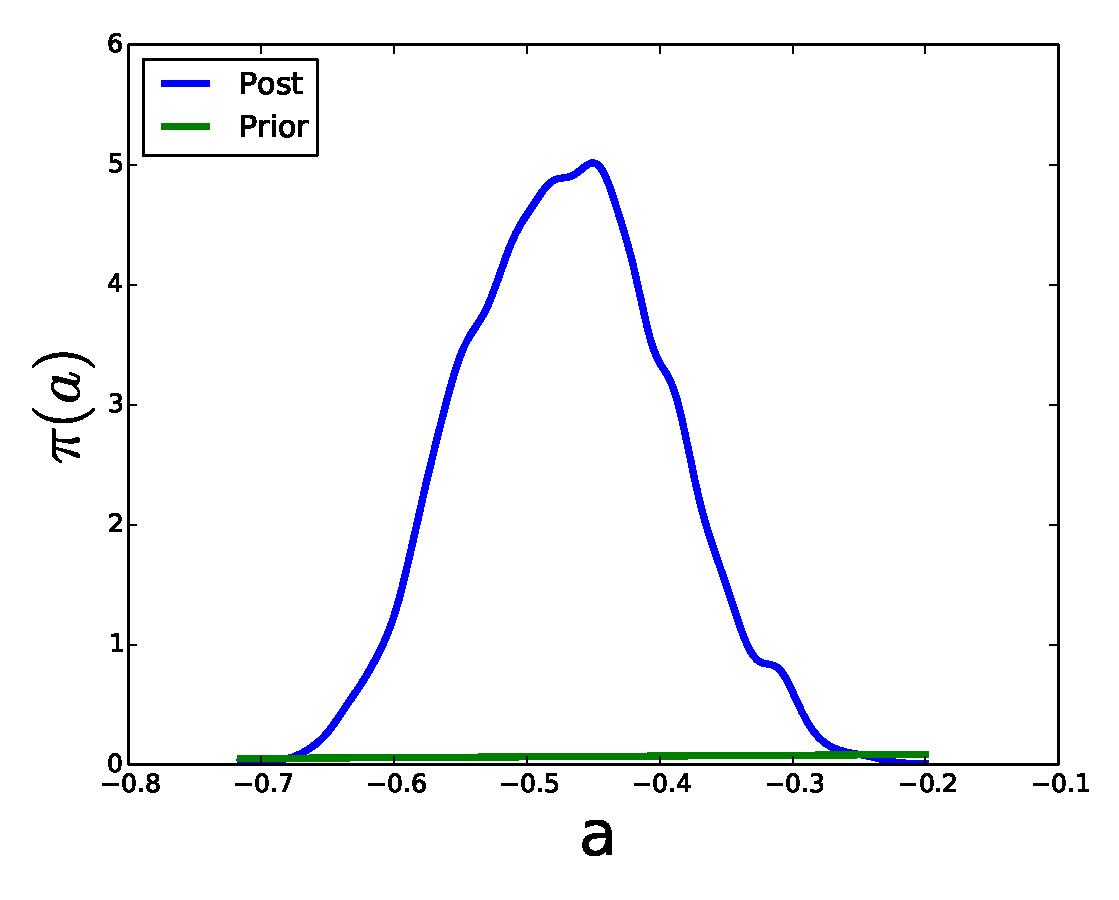
\includegraphics[width=8cm]{figs/a_post} 
\par\end{centering}

\caption{Prior and posterior probability function of parameter $\alpha$. }


\label{fig:Uc} 
\end{figure}


\begin{figure}[H]
\begin{centering}
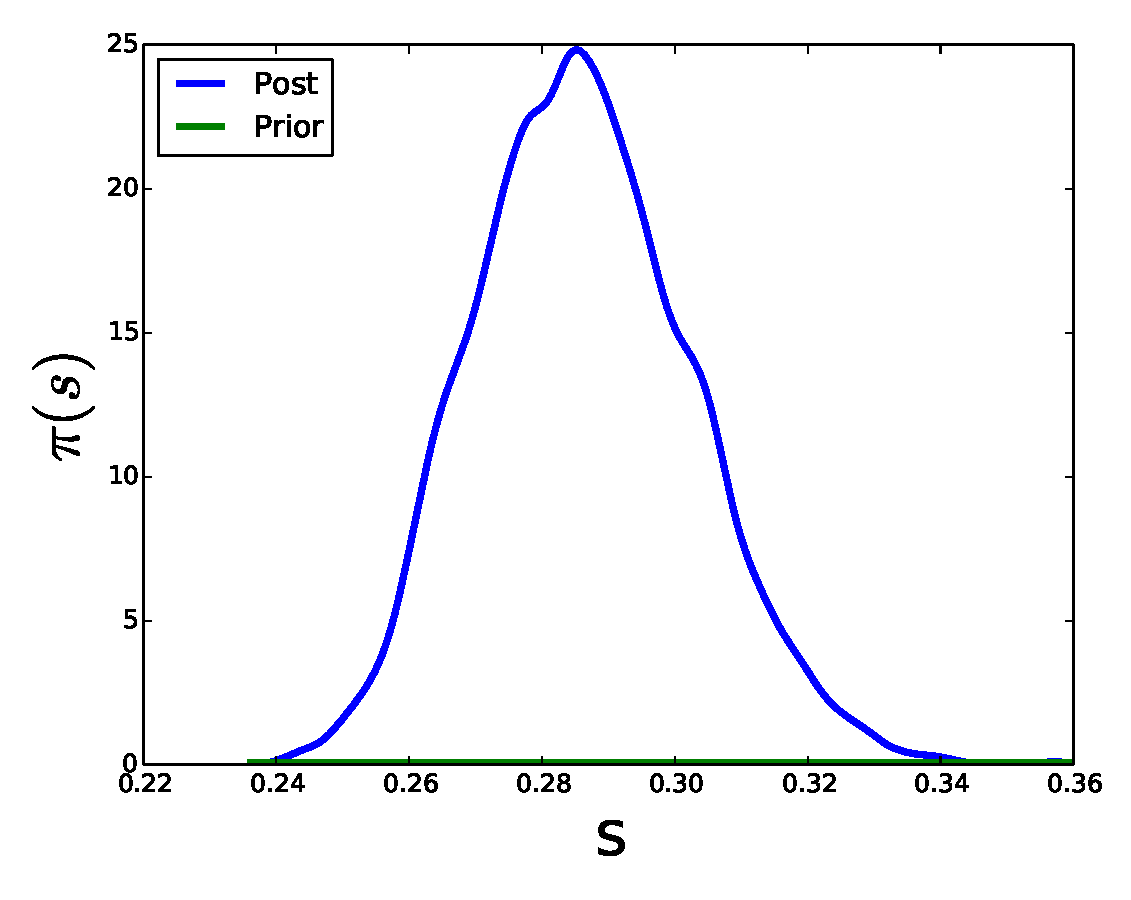
\includegraphics[width=8cm]{figs/s_post} 
\par\end{centering}

\caption{Prior and posterior probability distribution function of parameter
$\sigma$.}


\label{fig:Uc} 
\end{figure}


\begin{figure}[H]
\begin{centering}
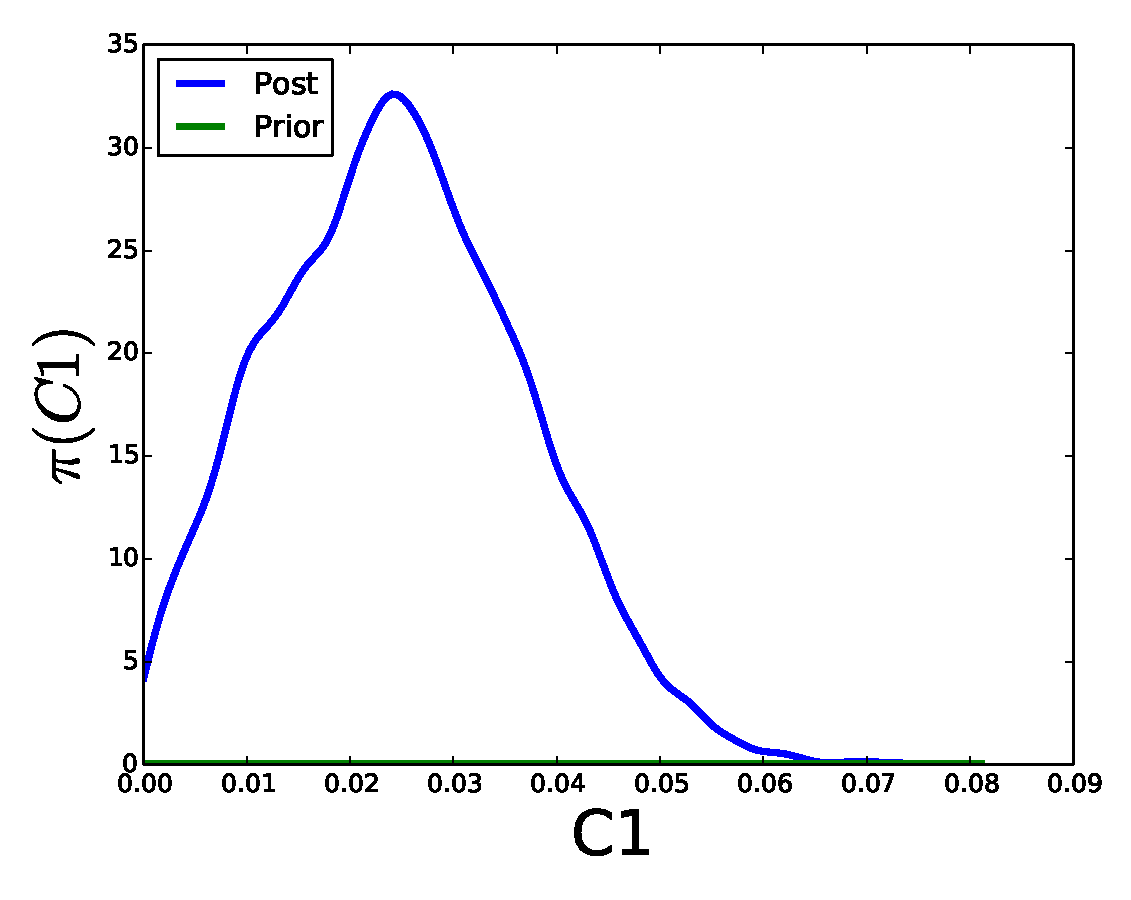
\includegraphics[width=8cm]{figs/C1_post} 
\par\end{centering}

\caption{Prior and posterior probability function of drag coefficient of bowling
ball $C_{d}1$. }


%Cd1


\label{fig:Uc} 
\end{figure}


\begin{figure}[H]
\begin{centering}
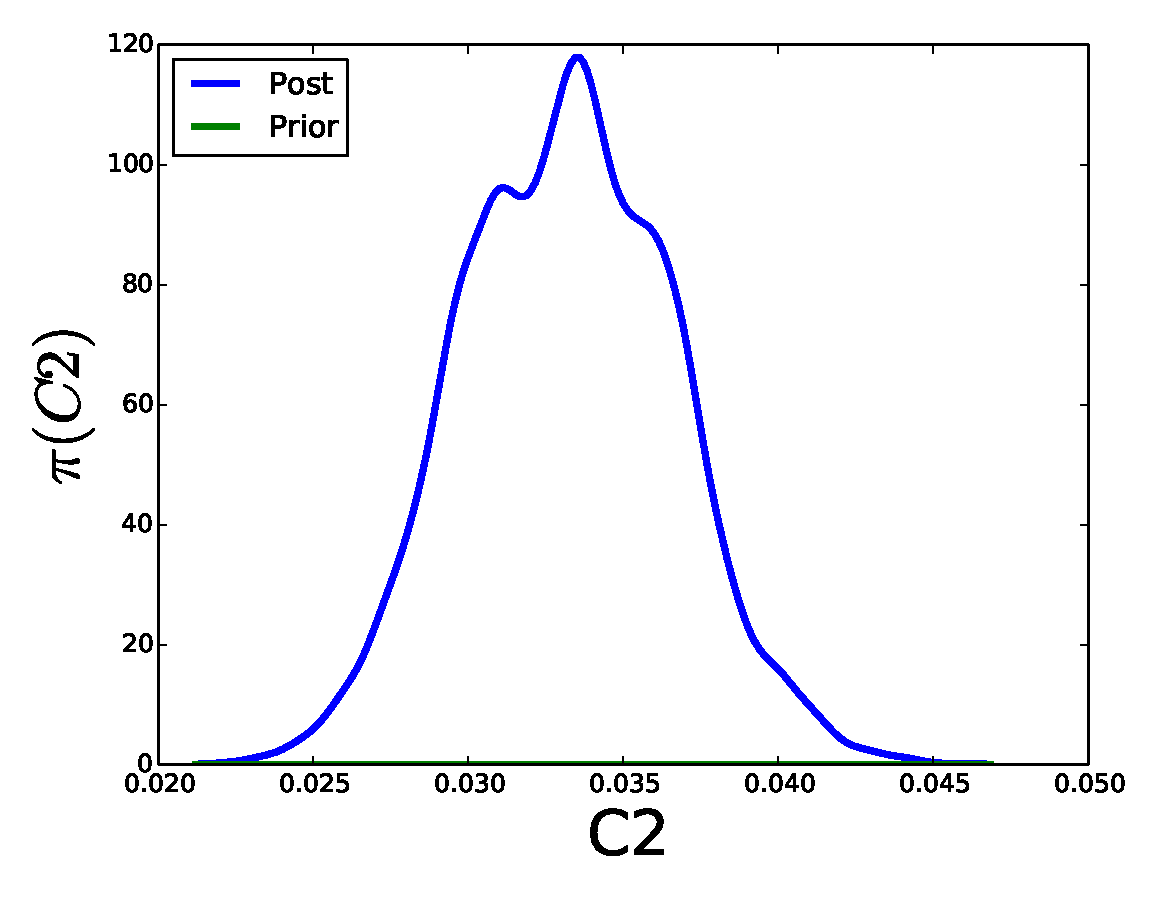
\includegraphics[width=8cm]{figs/C2_post} 
\par\end{centering}

\caption{Prior and posterior probability function of drag coefficient of basket
ball $C_{d}2$. }


%Cd1


\label{fig:Uc} 
\end{figure}



\section{Independent Samples}

Generate samples of the joint posterior distribution of the calibration
parameters for use in performing the validation calculations. Instead
of using every sample in the MCMC chain, you may want to take every
$n^{th}$ sample in the chain, so the samples will be closer to independent.
Again be sure to document what you do. You will need enough nearly
independent samples to accurately perform the Monte Carlo integrals
in (3).


\subsubsection*{Solution}

We created samples of the joint posterior distribution for $C_{d},\sigma$
and $\alpha$ using MCMC. The correlation between the samples were
measured using the program `Autoregressive process modeling tools'
(https://github.com/RhysU/ar). Table \ref{table:creatingindesamples}
shows the number of steps for each of the parameters required so that
the samples are independent (correlation fall below a specified value).
$C_{d}$ has by far the longest correlation between steps, more than
30 chain steps before decorrelation. 

An example of the arsel output is:
\begin{verbatim}
[nick@magus data]$ arsel -s < cd.dat | grep '#'
# absrho    true
# criterion CIC
# eff_N     32.751365129344251
# eff_var   0.12904055664629624
# gain      5.0428322668791719
# maxorder  512
# minorder  0
# mu        0.67116199032442436
# mu_sigma  0.062769462607289453
# N         1000
# AR(p)     71
# sigma2eps 0.024807597117980005
# sigma2x   0.12510055121028832
# submean   true
# T0        30.533078424386947
# window_T0 1
\end{verbatim}
Where $T_0$ presents the estimated envelope window of time of
correlation between samples. 

We generated a set of samples 300,000 long, and downsampled to 10,000
uncorrelated samples for the integrals. We then confirmed that these
samples were uncorrelated using arsel on the downsampled chains. Later,
we found that these 10k uncorrelated samples were complete overkill with
respect to the integration. Only a few hundred samples were needed to
compute the posterior distributions shown below, which are generally
quite smooth (and no further smoothing function or KDE was utilized afterwards). 

\begin{table}
\begin{centering}
\begin{tabular}{|c|c|}
\hline 
Parameter & Chain steps to decorrelation\tabularnewline
\hline 
\hline 
$C_{d}$ & 30.533078\tabularnewline
\hline 
$\sigma$ & 12.089690\tabularnewline
\hline 
$\alpha$ & 11.870957\tabularnewline
\hline 
\end{tabular}
\par\end{centering}

\caption{Creating independent samples.}


\label{table:creatingindesamples}
\end{table}



\section{Posterior of the observations}

Recall that the posterior distribution of an observation $y$, including
the uncertainty in the observation measurement is given by:

\begin{equation}
p\left(y|D,X\right)=\int_{\tilde{y}}\int_{\theta}p\left(y|\tilde{y},\theta,X\right)p\left(\tilde{y}|\theta,X\right)p\left(\theta|D,X\right)d\theta d\tilde{y}
\end{equation}


where $\tilde{y}$ is the unknown true value of the observable, and
$\theta$ is the vector of parameters. The conditional probabilities
in the integrand are:
\begin{itemize}
\item $p\left(y|\tilde{y},\theta,X\right)$ -- the probabilistic representation
of measurement error. It is conditioned on because of the calibration
parameters in the error model.
\item $p\left(\tilde{y}|\theta,X\right)$ -- this is the physical model,
which in our case is deterministic. Therefore, $p\left(\tilde{y}|\theta,X\right)=\delta\left(\tilde{y}-Y\left(\theta\right)\right)$
, where $Y\left(\theta\right)$ is the model predicted value of $\tilde{y}$
for given parameters , and $\delta\left(\right)$ is the Dirac delta
function. You made use of this fact when formulating the likelihood.
\item $p\left(\theta|D,X\right)$ is the posterior distribution of the parameters
obtained from the Bayesian calibration.
\end{itemize}
Because the model is deterministic, the $\tilde{y}$ integral can
be done trivially, further the samples of the parameters obtained
from the MCMC algorithm are samples from the posterior distribution
$p\left(\theta|D,X\right)$, so the $\theta$ integral can be performed
using a Monte Carlo method to obtain the approximation:

\begin{equation}
p\left(y|D,X\right)=\int_{\theta}p\left(y|Y\left(\theta\right),\theta,X\right)p\left(\theta|D,X\right)d\theta\approx\frac{1}{N}\sum_{j=1}^{N}p\left(y|Y\left(\theta_{j}\right),\theta_{j},X\right)
\end{equation}


where $\theta_{j}$ is the $j^{th}$ sample of $\theta$. Use this
Monte Carlo approximation, the samples from (2) and the measurement
error model developed for problem 2 to compute the posterior distribution
$p\left(y|D,X\right)$ for each observation of both balls considered
in problem 2. \textbf{Hint}: You can define a grid in $y$, with grid
points $y_{i}$ and evaluate the sum above for each $y_{i}$ . Be
sure to choose the grid spacing in $y$ to be fine enough to accurately
represent the distribution.


\subsubsection*{Solution}

In the general case, the posterior distribution of the observations~$y$
can be marginalized over the parameters~$\theta$ and the true value
of the observed quantity~$\tilde{y}$, 
\begin{align*}
p(y|D,X)=\int_{\tilde{y}}\int_{\theta}p(y,\tilde{y},\theta|D,X)\, d\theta d\tilde{y}.
\end{align*}
 We can then apply Bayes' theorem twice to get 
\begin{align*}
p(y|D,X) & =\int_{\tilde{y}}\int_{\theta}p(y|\tilde{y},\theta,D,X)p(\tilde{y},\theta|D,X)\, d\theta d\tilde{y}\\
 & =\int_{\tilde{y}}\int_{\theta}p(y|\tilde{y},\theta,D,X)p(\tilde{y}|\theta,D,X)p(\theta|D,X)\, d\theta d\tilde{y}.
\end{align*}
 We can now simplify this expression a bit more by noticing that the
first two conditional probability density functions~(pdf) do not
depend on the observed quantities~$D$. We end up with the expression
found in the problem statement 
\begin{equation}
p(y|D,X)=\int_{\tilde{y}}\int_{\theta}p(y|\tilde{y},\theta,X)p(\tilde{y}|\theta,X)p(\theta|D,X)\, d\theta d\tilde{y}.\label{eq:postobsfull}
\end{equation}
 In this exercise, we did not assume any model inadequacy. Therefore,
the second pdf inside the integral is simply given by the deterministic
physical model, i.e. 
\[
p(\tilde{y}|\theta,X)=\delta(\tilde{y}-Y(\theta)),
\]
 where $Y$ is the deterministic physical model. Then expression~\ref{eq:postobsfull}
simplifies more to 
\begin{equation}
p(y|D,X)=\int_{\theta}p(y|Y(\theta),\theta,X)p(\theta|D,X)\, d\theta,\label{eq:postobs}
\end{equation}
 where $p(y|Y(\theta),\theta,X)$ is the observational model and $p(\theta|D,X)$
is the posterior distribution coming from the calibration.

Applying a Monte-Carlo approximation we evaluate integral~(\ref{eq:postobs})
thanks to the samples drawn in question~2. This gives 
\begin{equation}
p(y|D,X)\approx\frac{1}{N}\sum_{i=1}^{N}p(y|Y(\theta_{i}),\theta_{i},X).\label{eq:postobsmc}
\end{equation}
 The variable~$y$ represents the observation and could be as such
understood as a vector of all the observations made. However multi-dimensional
model validation is cumbersome and instead we'll treat each observation
separately. For each ball, we had the results from two experiments.
Let's number these experiments and call the observations $y^{1}(t),y^{2}(t),y^{3}(t),y^{4}(t)$.
In each experiment, the ball position was only recorded at a discrete
number of times, we in fact we are dealing with the data 
\[
y^{1}(t_{1}^{1}),y^{1}(t_{2}^{1}),\ldots,y^{1}(t_{N_{1}}^{1}),y^{2}(t_{1}^{2}),\ldots,y^{2}(t_{N_{2}}^{2}),\ldots,y^{4}(t_{N_{4}}^{4}).
\]
 And therefore for any $i=1,\ldots,4$ and $j=1,\ldots,N_{i}$, let
$y^{i,j}:=y^{i}(t_{j}^{i})$. We then want to evaluate 
\[
p(y^{i,j}|D,X)\approx\frac{1}{N}\sum_{s=1}^{N}p(y^{i,j}|Y(\theta_{s}),\theta_{s},X).
\]
 We are going to evaluate that sum on a grid. For storage efficiency,
each observation will have its own grid centered around a reasonable
value (to be defined later). The grid is then defined as 
\[
y_{k}^{i,j}=y_{c}^{i,j}+k\Delta y,\quad\forall k\in\{-m^{i,j},m^{i,j}\}.
\]
 For a given $i=1,\ldots,4$ and $j=1,\ldots,N_{i}$, we are going
to store the values of 
\[
\frac{1}{N}\sum_{s=1}^{N}p(y^{i}(t_{j}^{i})=y_{k}^{i,j}|Y(\theta_{s}),\theta_{s},X),\quad\forall k\in\{-m^{i,j},m^{i,j}\}.
\]
 We can now write down explicitly the formula for that quantity. In
the group project~\#2, we defined the measurement error as a multivariate
Gaussian with mean and covariance depending on the calibration parameters~$\alpha$
and $\sigma$. But here we only care about the marginalized distribution
of a single observation. Fortunately, marginalized distributions of
Gaussian are also Gaussian with mean and covariance being given by
the restriction of the multivariate mean and covariance to the variables
of interest. In our case, we end up with a Gaussian of mean $\alpha t_{j}^{i}$
and covariance $\sigma^{2}$. Let's call $y_{c}^{i,j}$ the computed
solution of the ball drop without noise. We can therefore write 
\[
y^{i,j}=y_{c}^{i,j}+\varepsilon,
\]
 with $\varepsilon\sim\mathcal{N}(\alpha t_{j}^{i},\sigma^{2})$.
Then we store at each grid point 
\[
\frac{1}{N}\frac{1}{\sqrt{2\pi}\sigma}\sum_{s=1}^{N}e^{-(y_{k}^{i,j}-y_{c}^{i,j}-\alpha t_{j}^{i})^{2}/2\sigma^{2}},\quad\forall k\in\{-m^{i,j},m^{i,j}\}.
\]



\section{Credibility}

For each observation, compute the the credibility $1-\beta$, where
the datum is the maximum or minimum value of a $\beta-$credibility
set. You may use either an HPD or quantile credibility set. Plot these
credibility values as a function of time for the four ball drops considered.
\textbf{Hint}: you can approximate the required integrals using the
grid of values obtained in 3) and a quadrature rule, such as trapezoidal
rule.


\subsubsection*{Solution}

The credibility of a given distribution is defined as alpha = 1 \textendash{}
beta, where beta = integral(P(y)dy). In this project, we made the
decision to 
use the HPD method to compute the credibility. HPD was selected because
we did not know if the distributions would be skewed (in reality, they
did not appear to have been strongly skewed) and HPD would provide a
more robust estimate than the quartile analysis in this case. 
In the figures below, we
plot the credibility as a function of time for the 4 sets of measurements
(2 basket ball and 2 bowling ball). As one can clearly observe from
the figures, the data seems to be credible (wrt the model) only for
the first fractions of a second and then becomes incredible later on. In other
words, this means the predictions of the model are quickly inconsistent with the
observations. This figure depicts the credibility interval for the first
data set with the basketball, but all data sets and balls were
qualititively similar. 

\begin{figure}[H]
\begin{centering}
\includegraphics[width=8cm]{figs/credibility} 
\par\end{centering}
\caption{Credibility as a function of time.}

\label{fig:Uc} 
\end{figure}

For all the datasets, after 1.5 seconds, the HPD credibility is assessed
as exceeding low, at less than $1e-5$. Around 2.5 seconds, every data
set is completely implausible, with credibilities assessed at less than
$1e-10$. In summary, the credibility decreases as a function of time,
and after a few seconds, the predictions of our model are completely
inconsistent with the observations. 

\section{Validation test}

Choose two or more data points for each drop (including those with
the highest and lowest credibility), and plot the predicted posterior
distribution of the observation $p\left(y|D,X\right)$ along with
the value of the actual observation.


\subsubsection*{Solution}

The plots below show the best and the worst credibility intervals
along with credibility at few other time steps. The cases where $\beta$
falls within distribution give credence that the model is plausible \textendash{}
i.e. the model prediction is not inconsistent with the data. For the
values far outside the distribution, the model prediction is
inconsistent with the data, which certainly implies that we cannot trust
the model predictions to match those of observations. This is evidence
for an invalidation of the model, but further investigations would be
necessary to actually determine what is the ultimate cause of the
inconsistency (such as overly optimistic observation error bounds,
inaccurate scenario measurements, etc.).


\subsection{Ball drop - 1 (Basket Ball) }

\begin{figure}[H]
\begin{centering}
\subfigure[]{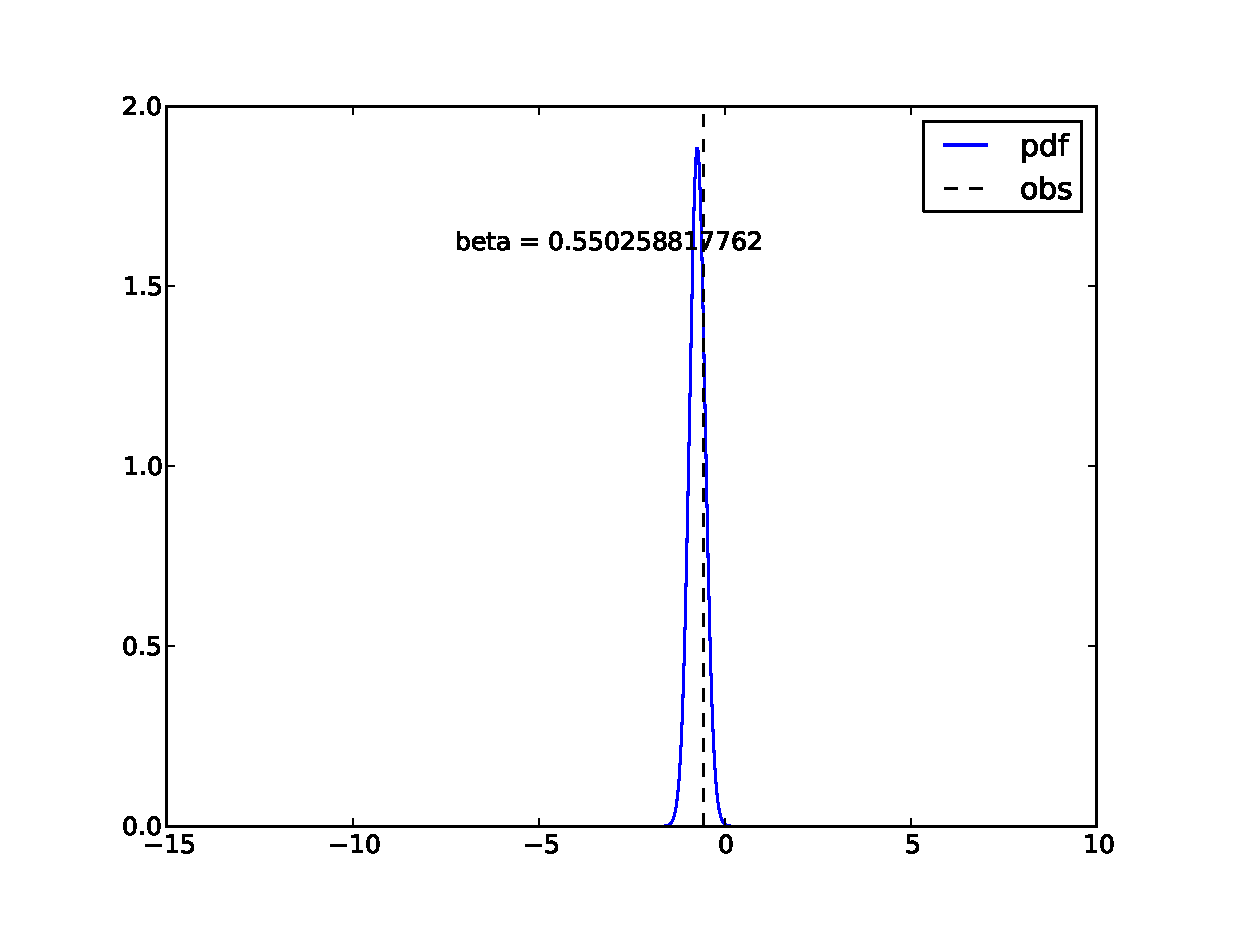
\includegraphics[width=6cm]{figs/Basket_Ball_1_5}}\,\,\,\subfigure[]{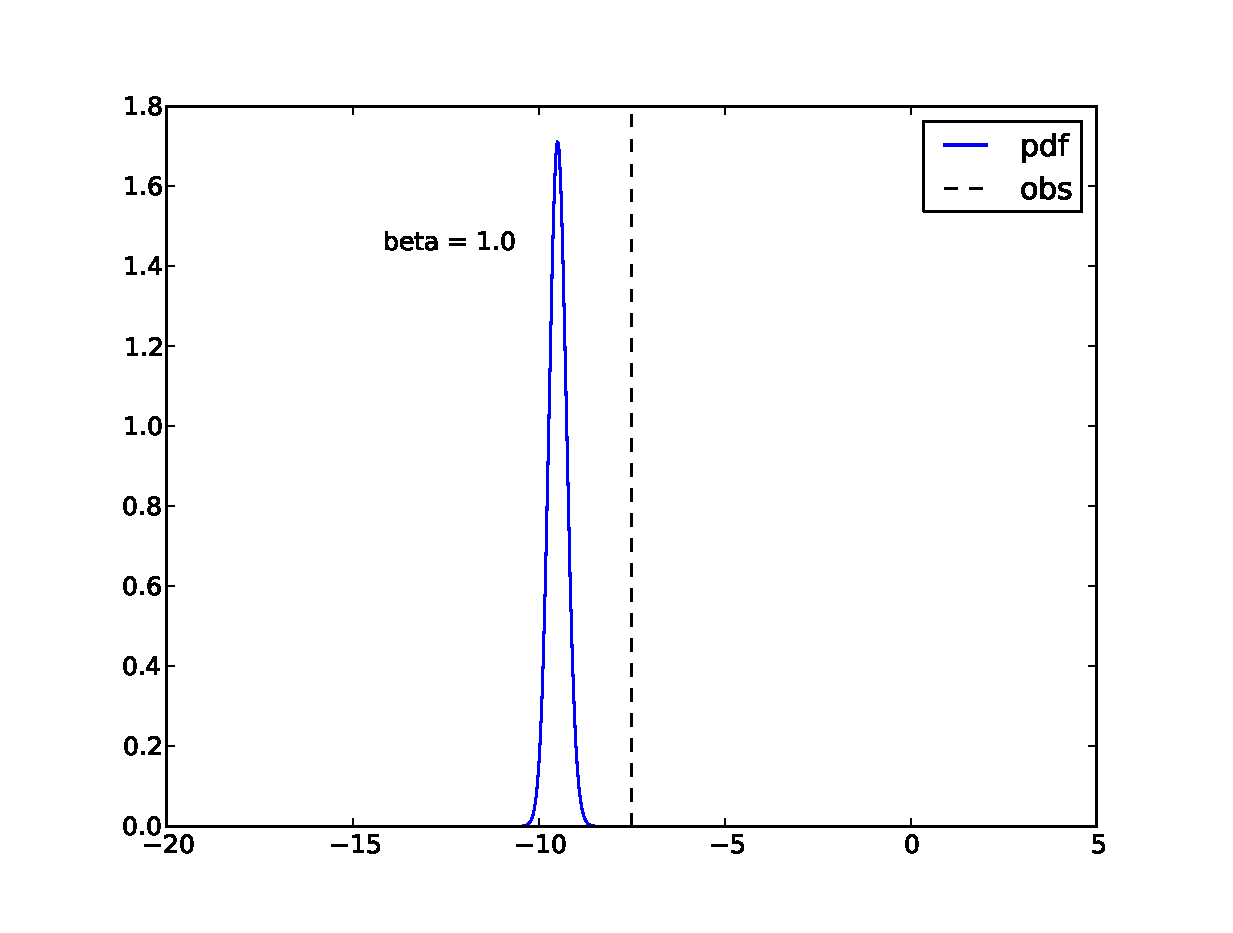
\includegraphics[width=6cm]{figs/Basket_Ball_1_20}}\,\,\,\subfigure[]{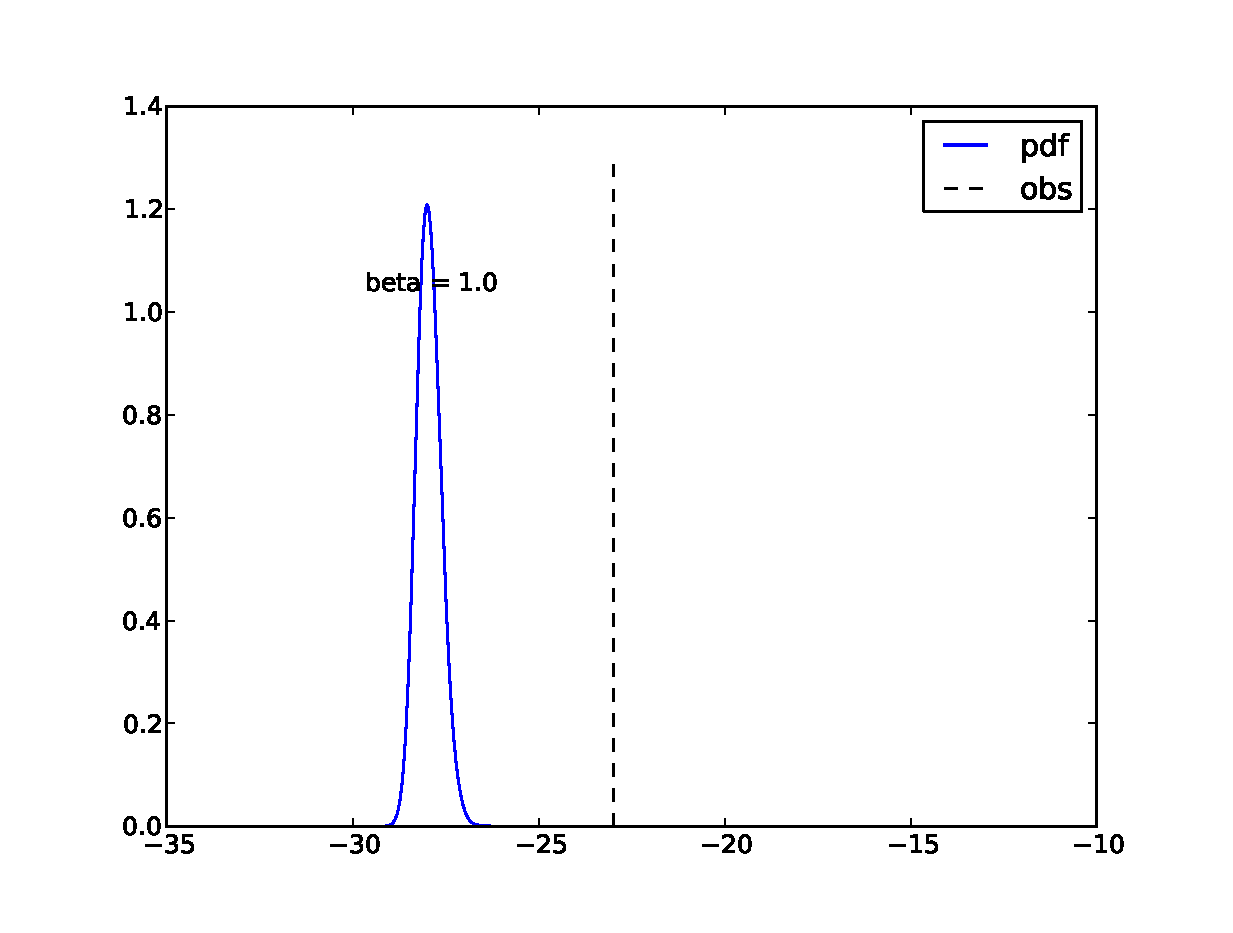
\includegraphics[width=6cm]{figs/Basket_Ball_1_35}}
\par\end{centering}

\caption{Predicted posterior distribution at time (a) $t=5$ (b) $t=20$ and
(c) $t=35$ secs vs the actual observation}


\label{balldrop1t5}

\end{figure}


\begin{figure}[H]
\begin{centering}
\subfigure[]{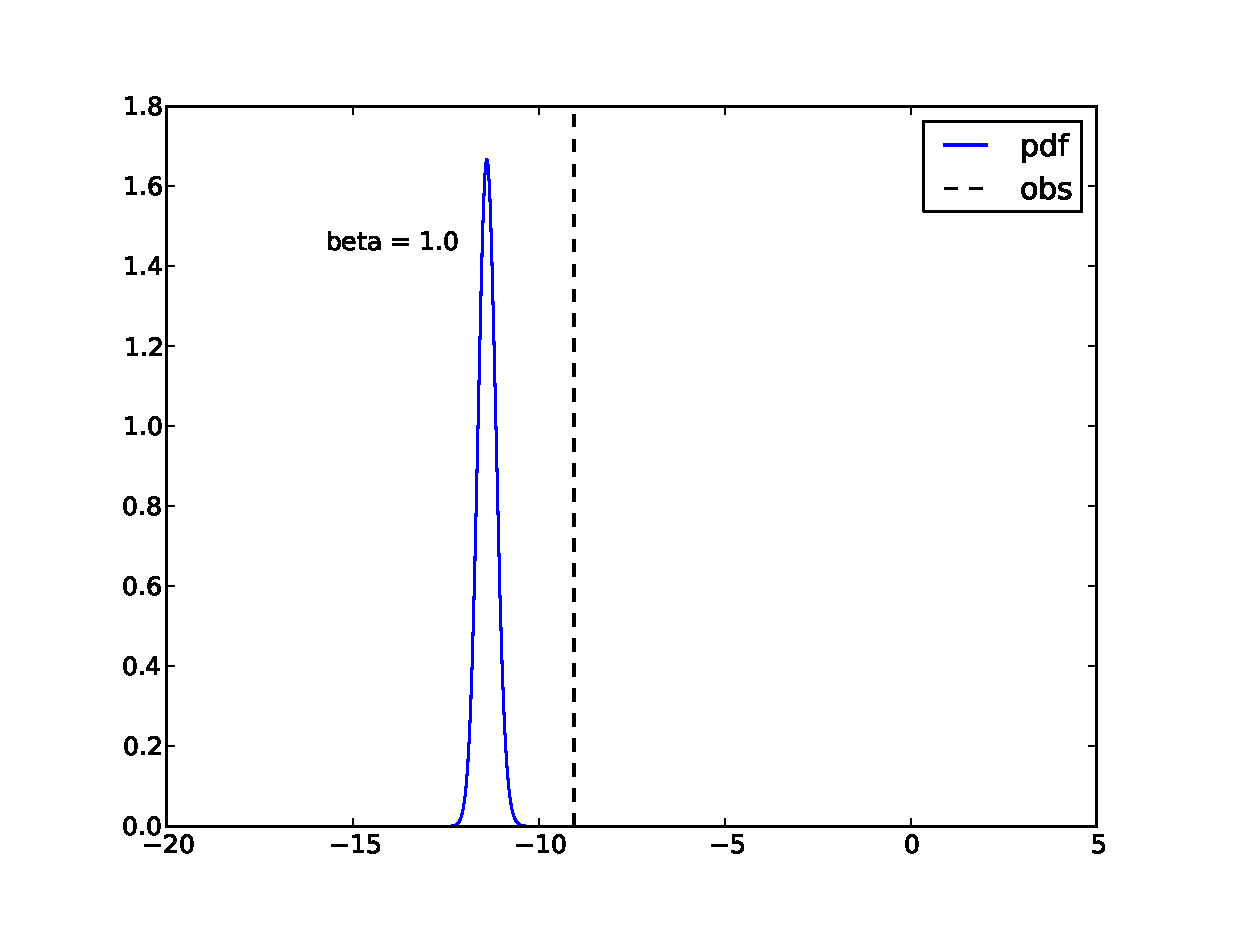
\includegraphics[width=6cm]{figs/Basket_Ball_1_maxbeta22}}\,\,\,\subfigure[]{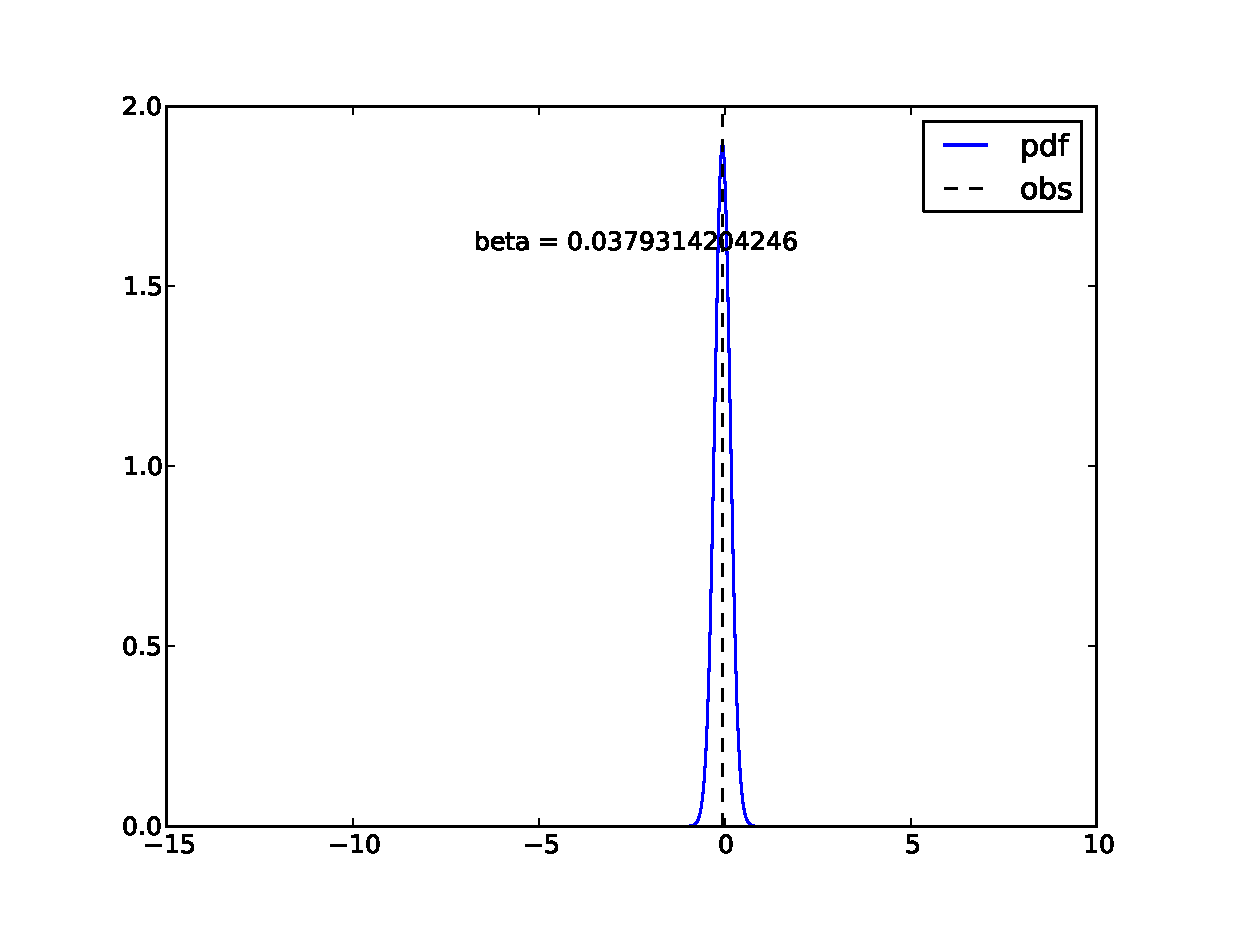
\includegraphics[width=6cm]{figs/Basket_Ball_1_minbeta1}}
\par\end{centering}

\caption{Predicted posterior distribution at (a) maximum $\beta$ (b) minimum
$\beta$}


\label{balldrop1t5-3}
\end{figure}



\subsection{Ball drop - 2 (Basket Ball)}

\begin{figure}[H]
\begin{centering}
\subfigure[]{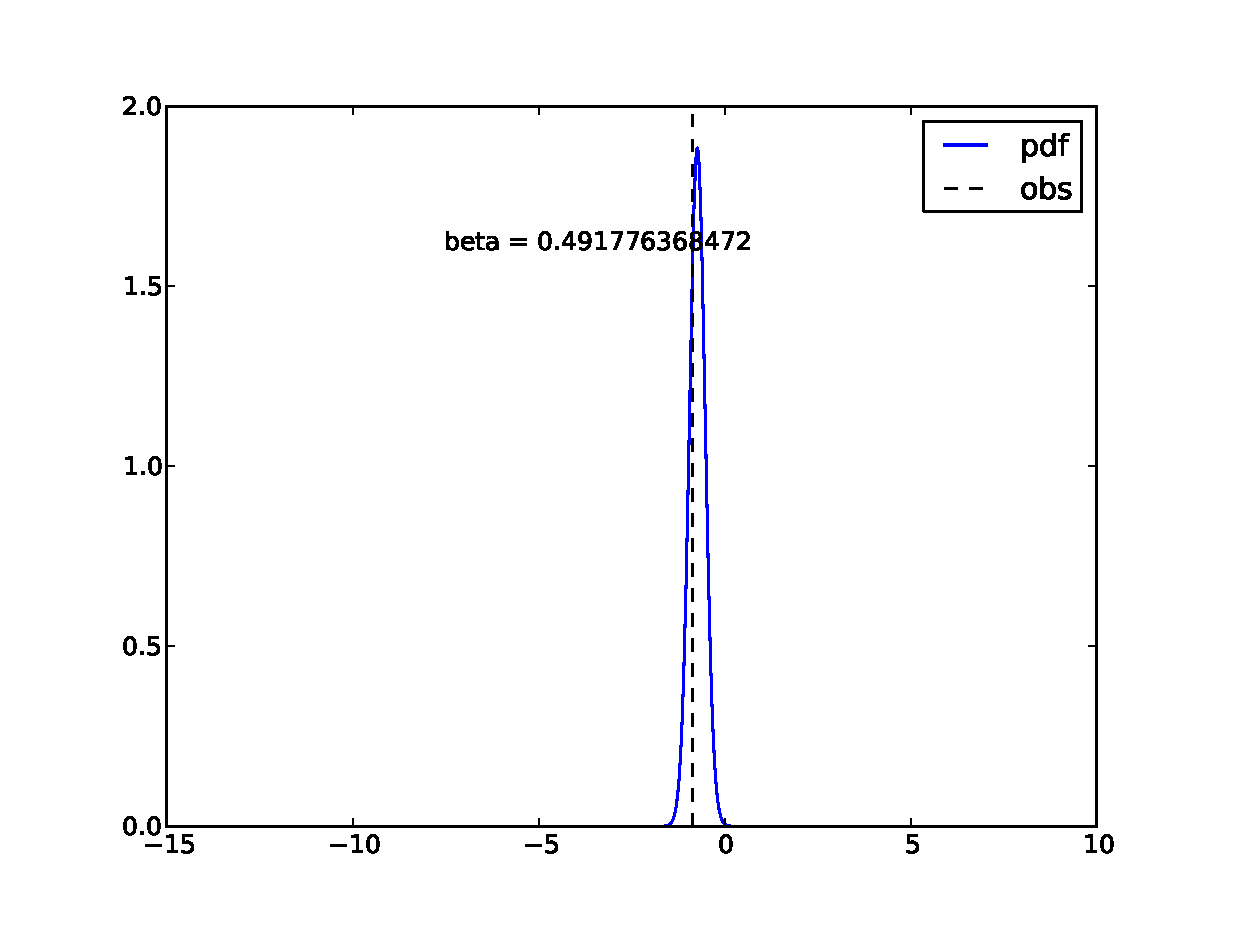
\includegraphics[width=6cm]{figs/Basket_Ball_2_5}}\,\,\,\subfigure[]{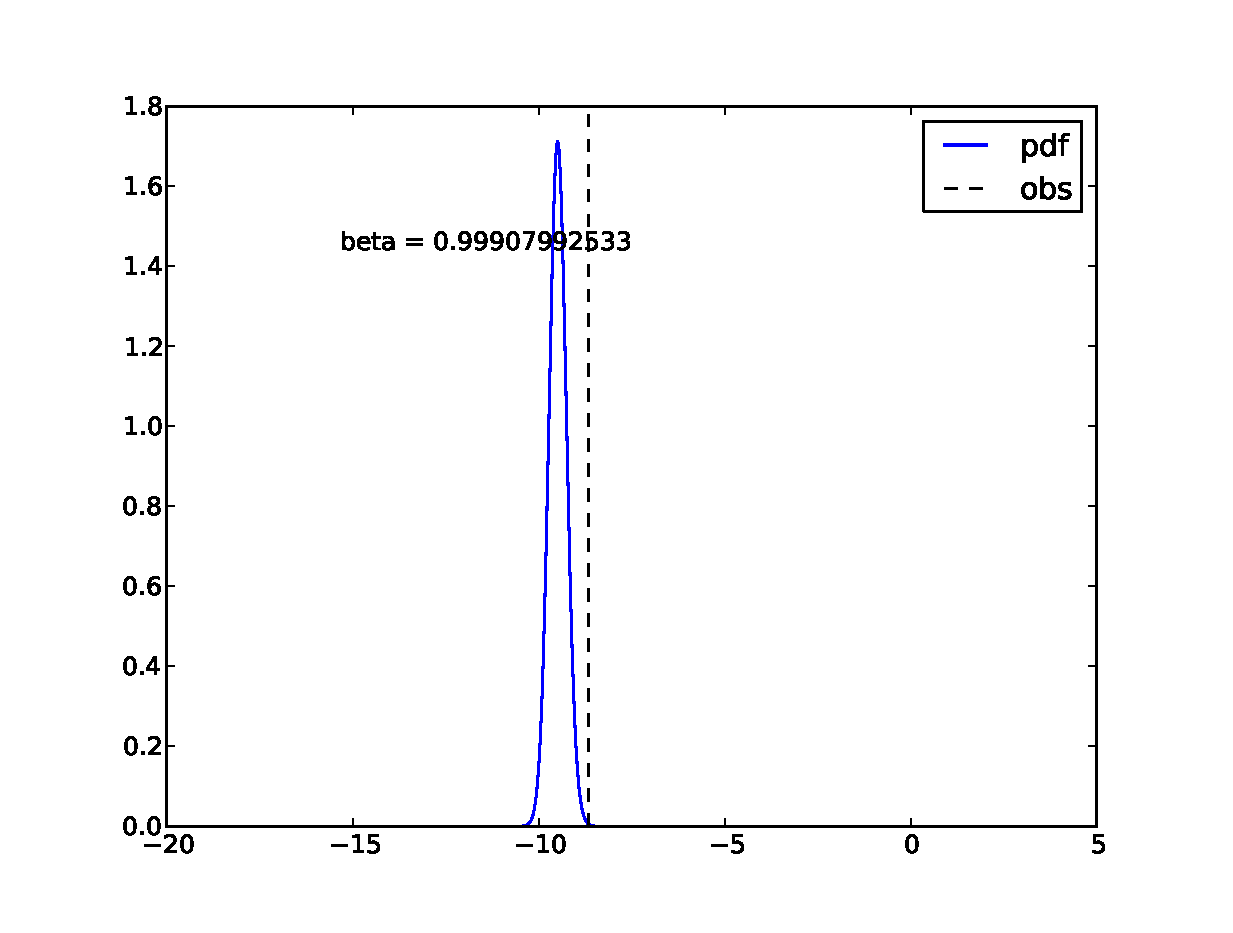
\includegraphics[width=6cm]{figs/Basket_Ball_2_20}}\,\,\,\subfigure[]{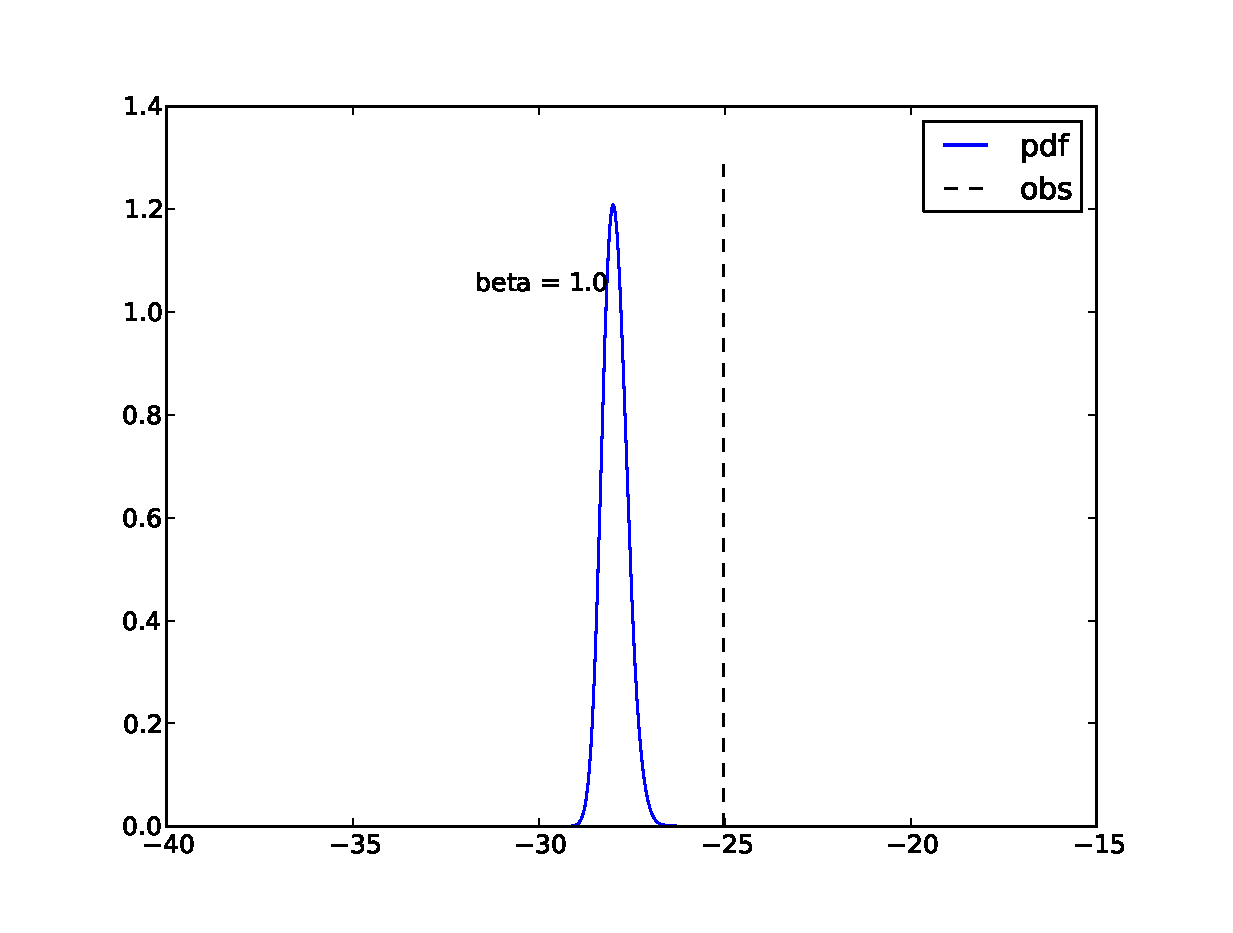
\includegraphics[width=6cm]{figs/Basket_Ball_2_35}}
\par\end{centering}

\caption{Predicted posterior distribution at time (a) $t=5$ (b) $t=20$ and
(c) $t=35$ secs vs the actual observation}


\label{balldrop1t5-1}
\end{figure}


\begin{figure}[H]
\begin{centering}
\subfigure[]{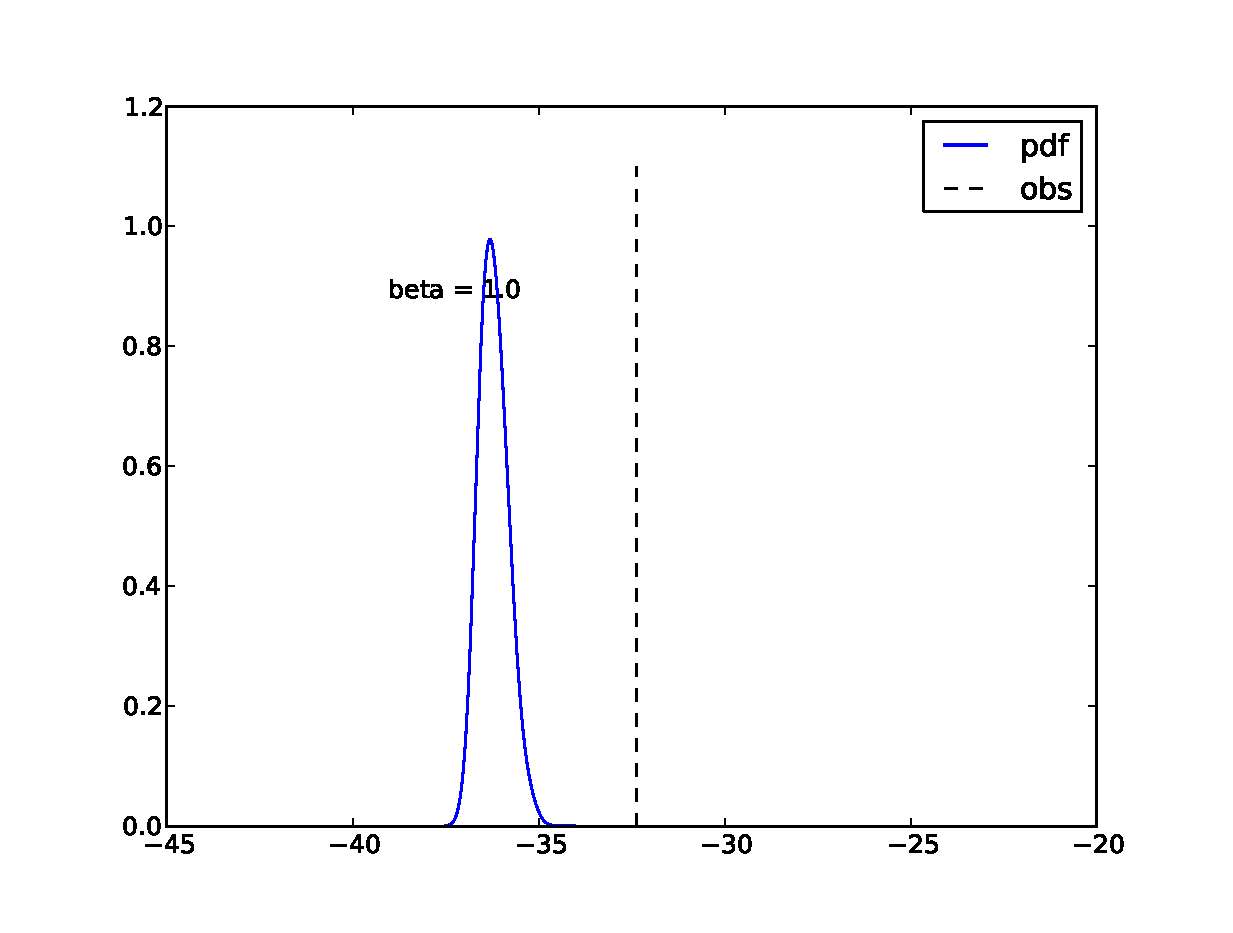
\includegraphics[width=6cm]{figs/Basket_Ball_2_maxbeta40}}\,\,\,\subfigure[]{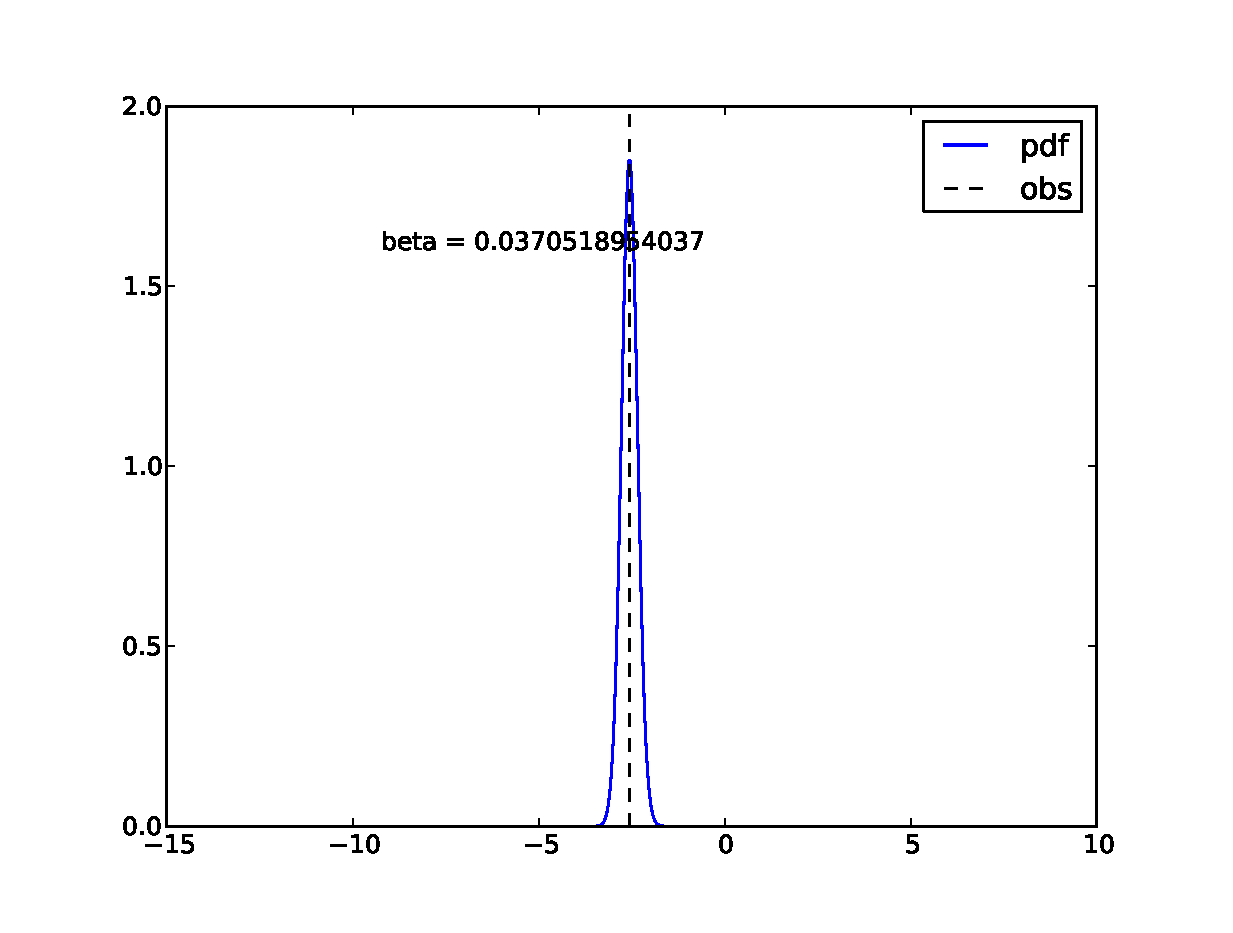
\includegraphics[width=6cm]{figs/Basket_Ball_2_minbeta10}}
\par\end{centering}

\caption{Predicted posterior distribution at (a) maximum $\beta$ (b) minimum
$\beta$}


\label{balldrop1t5-3-1}
\end{figure}



\subsection{Ball drop - 1 (Bowling Ball)}

\begin{figure}[H]
\begin{centering}
\subfigure[]{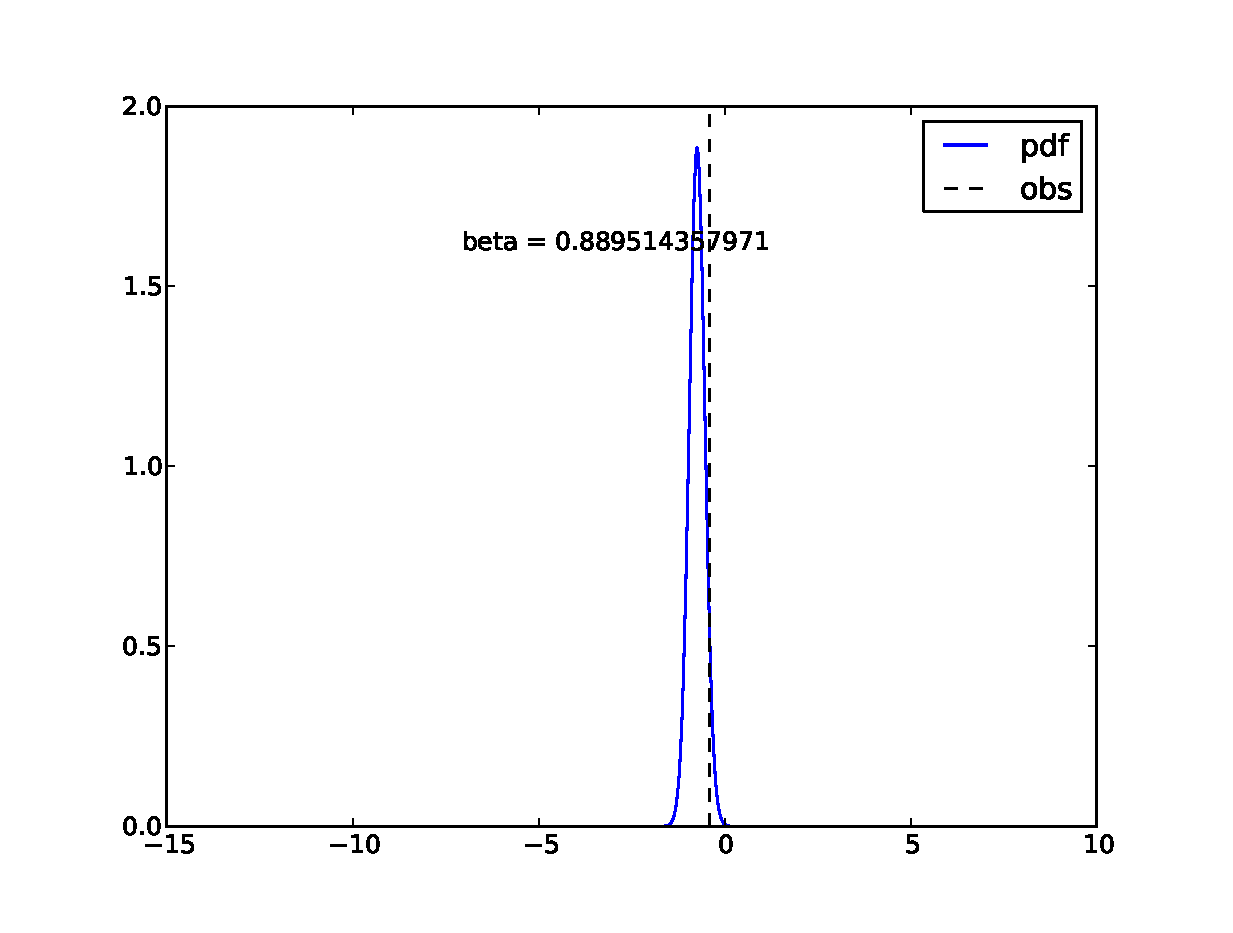
\includegraphics[width=6cm]{figs/Bowling_Ball_1_5}}\,\,\,\subfigure[]{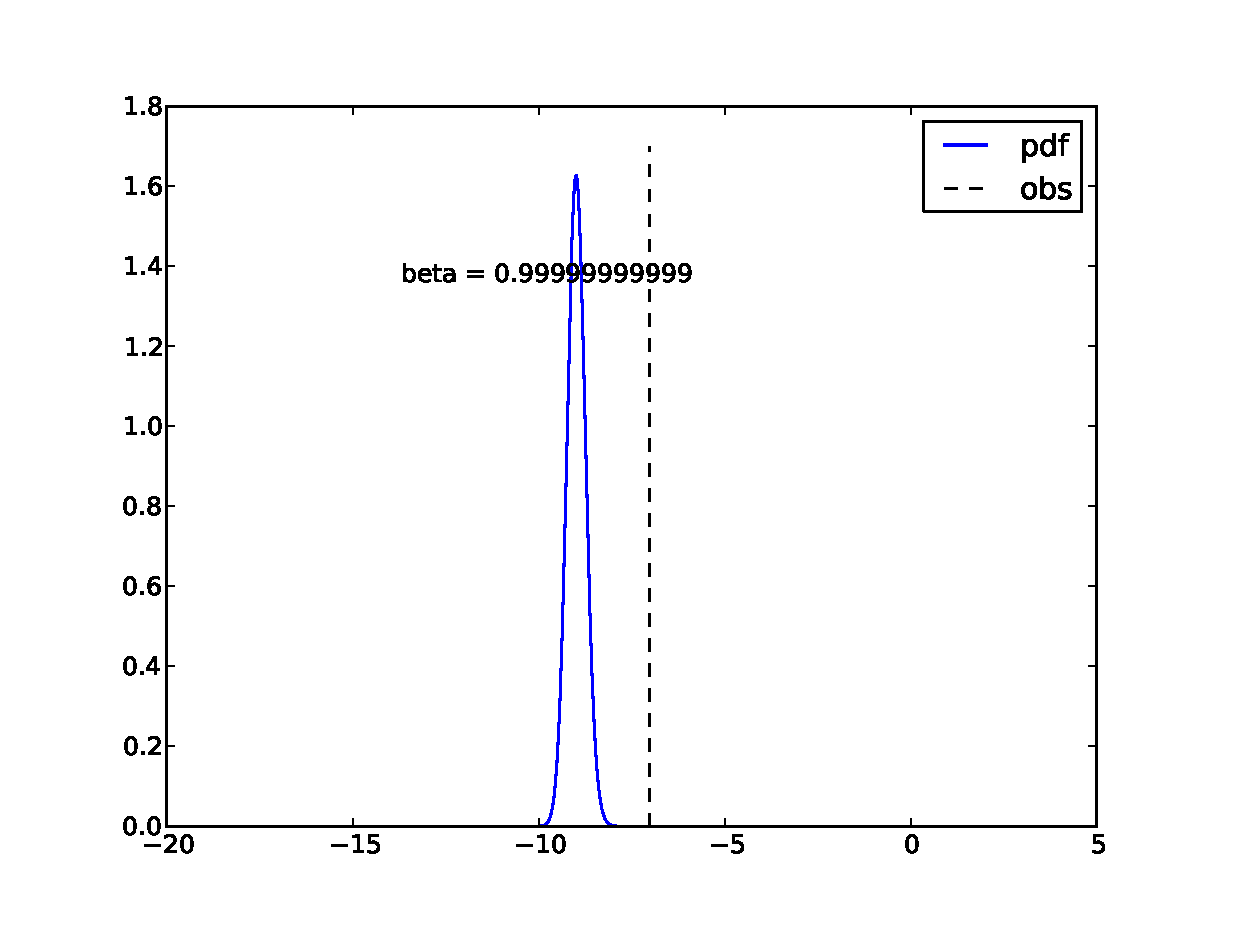
\includegraphics[width=6cm]{figs/Bowling_Ball_1_20}}\,\,\,\subfigure[]{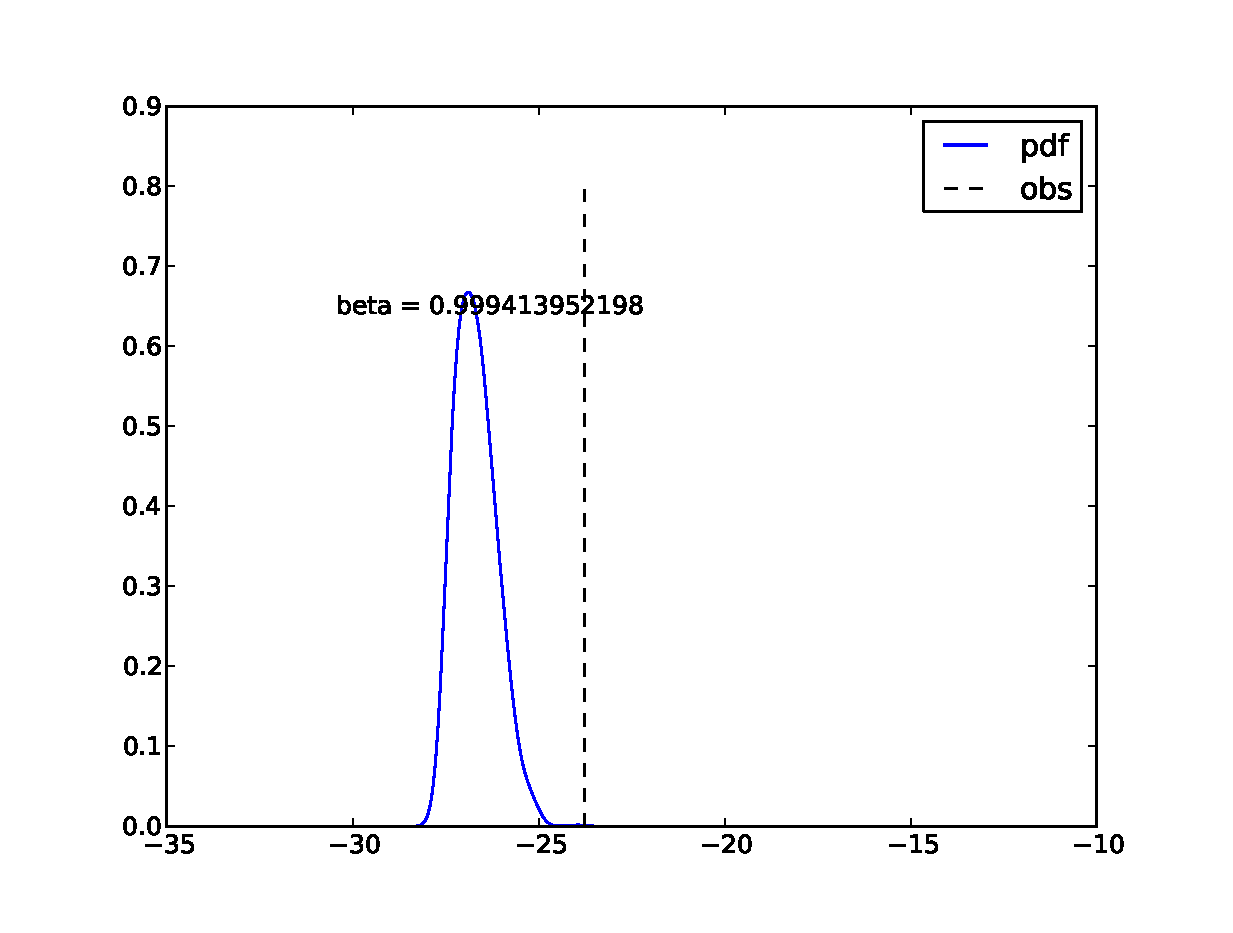
\includegraphics[width=6cm]{figs/Bowling_Ball_1_35}}
\par\end{centering}

\caption{Predicted posterior distribution at time (a) $t=5$ (b) $t=20$ and
(c) $t=35$ secs vs the actual observation}


\label{balldrop1t5-2}
\end{figure}


\begin{figure}[H]
\begin{centering}
\subfigure[]{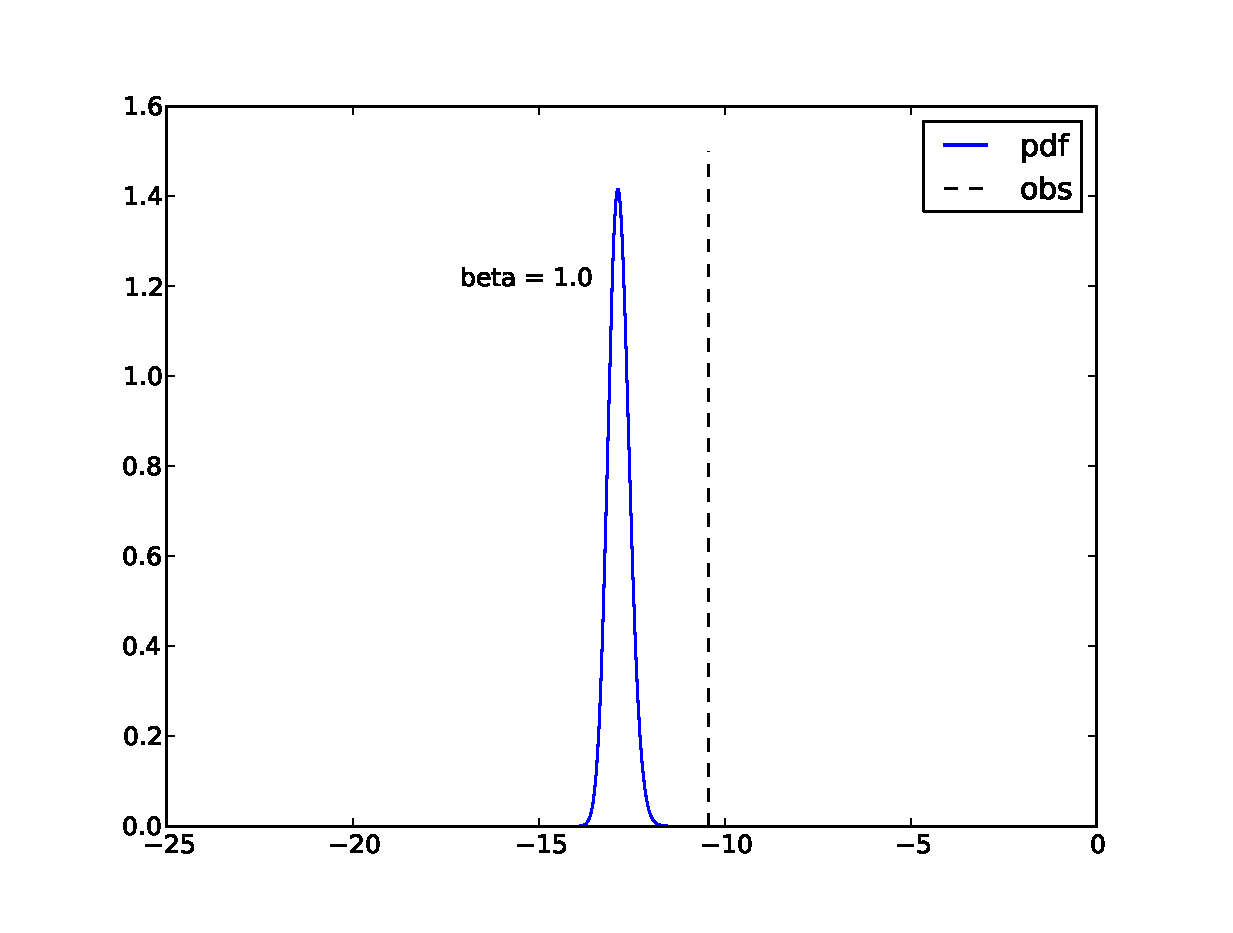
\includegraphics[width=6cm]{figs/Bowling_Ball_1_maxbeta24}}\,\,\,\subfigure[]{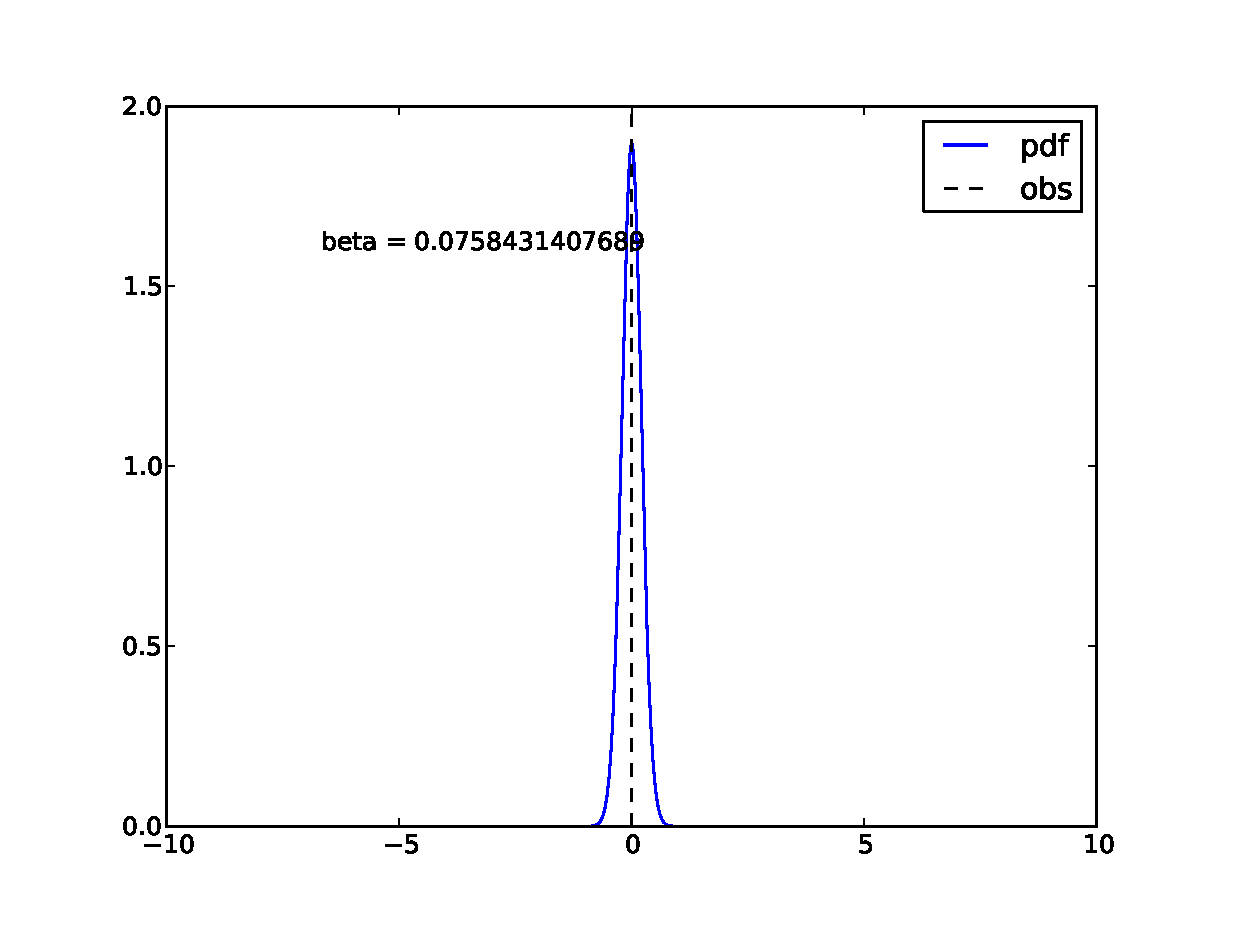
\includegraphics[width=6cm]{figs/Bowling_Ball_1_minbeta0}}
\par\end{centering}

\caption{Predicted posterior distribution at (a) maximum $\beta$ (b) minimum
$\beta$}


\label{balldrop1t5-3-2}
\end{figure}



\subsection{Ball drop - 2 (Bowling Ball)}

\begin{figure}[H]
\begin{centering}
\subfigure[]{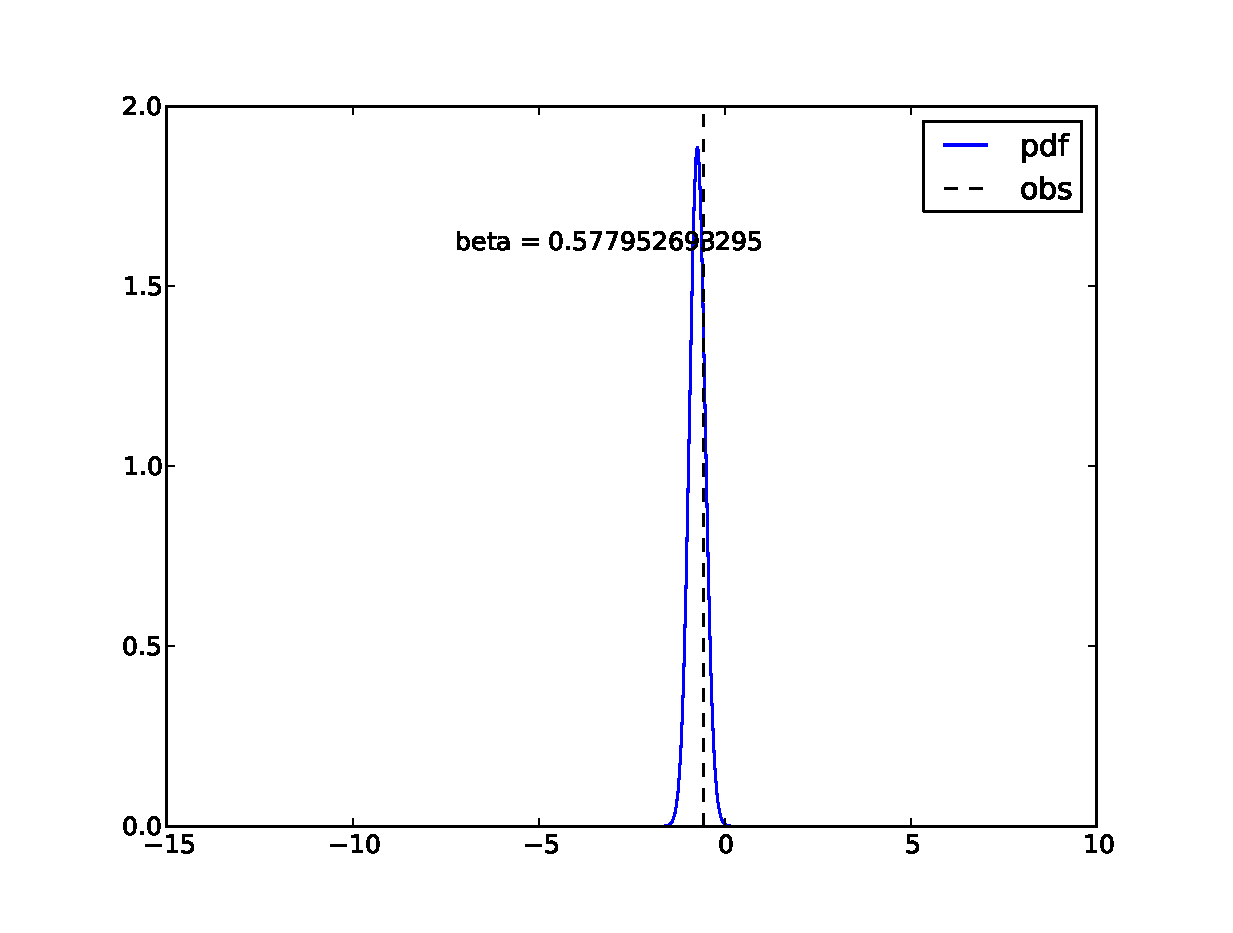
\includegraphics[width=6cm]{figs/Bowling_Ball_2_5}}\,\,\,\subfigure[]{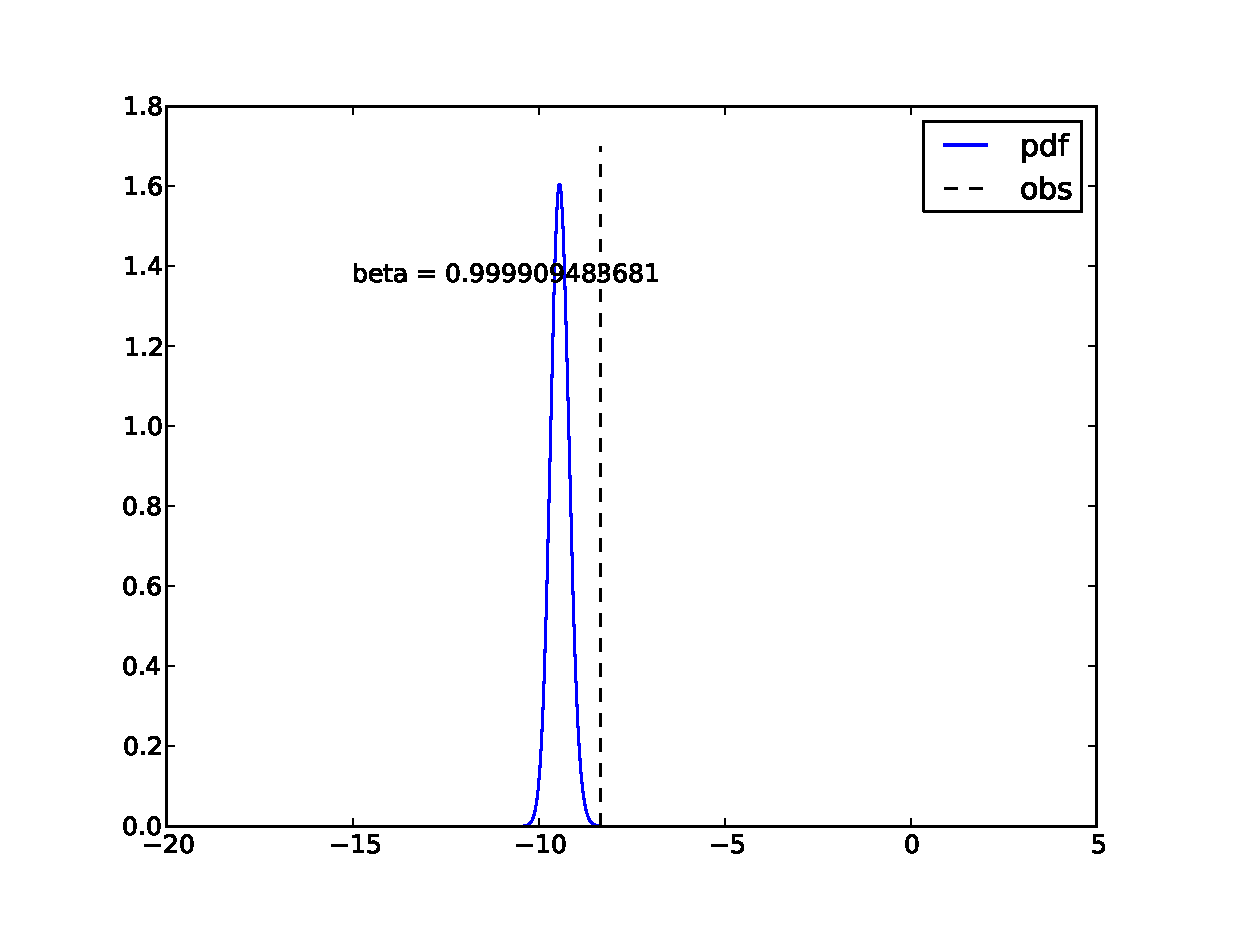
\includegraphics[width=6cm]{figs/Bowling_Ball_2_20}}\,\,\,\subfigure[]{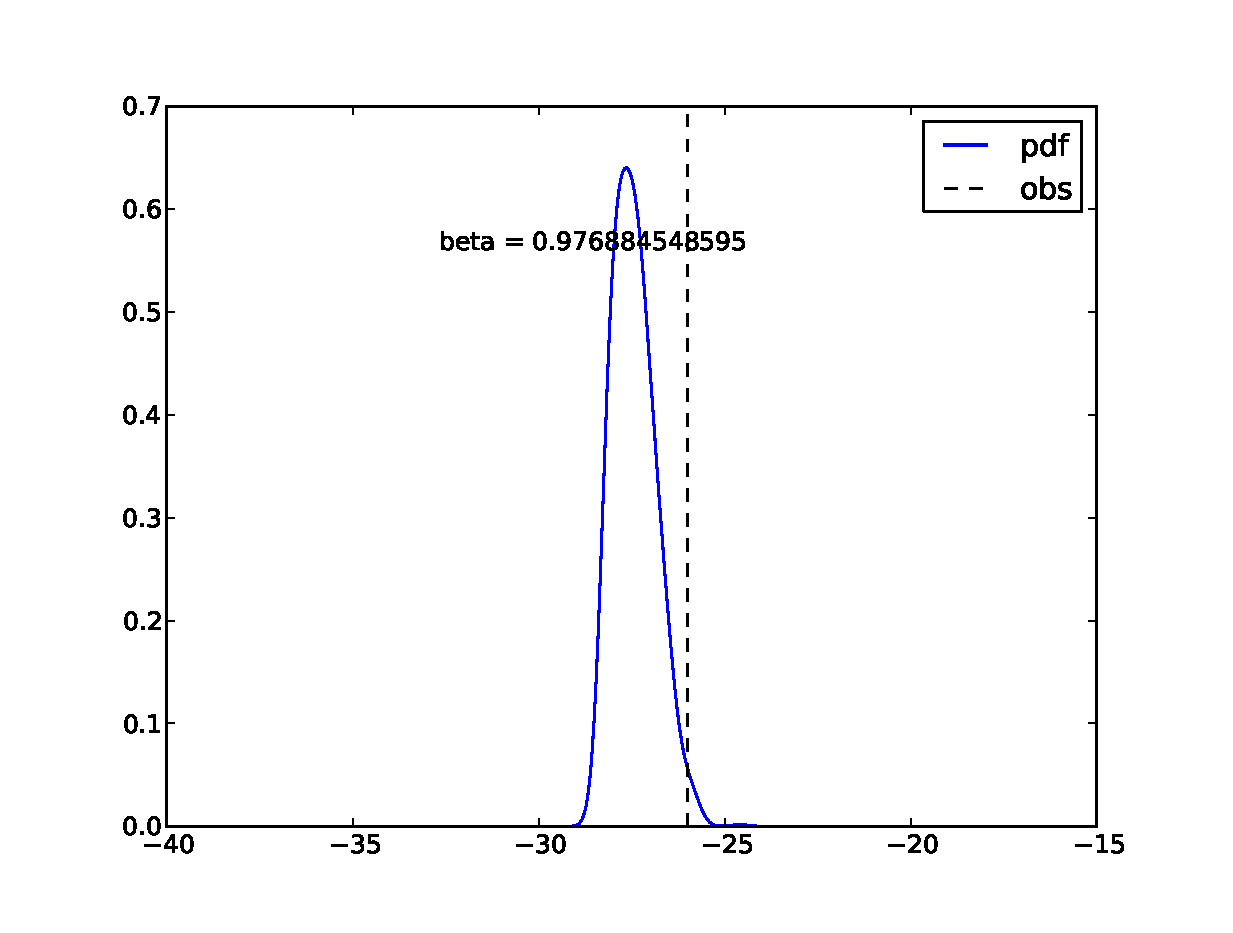
\includegraphics[width=6cm]{figs/Bowling_Ball_2_35}}
\par\end{centering}

\caption{Predicted posterior distribution at time (a) $t=5$ (b) $t=20$ and
(c) $t=35$ secs vs the actual observation}


\label{balldrop1t5-4}
\end{figure}



\begin{figure}[H]
\begin{centering}
\subfigure[]{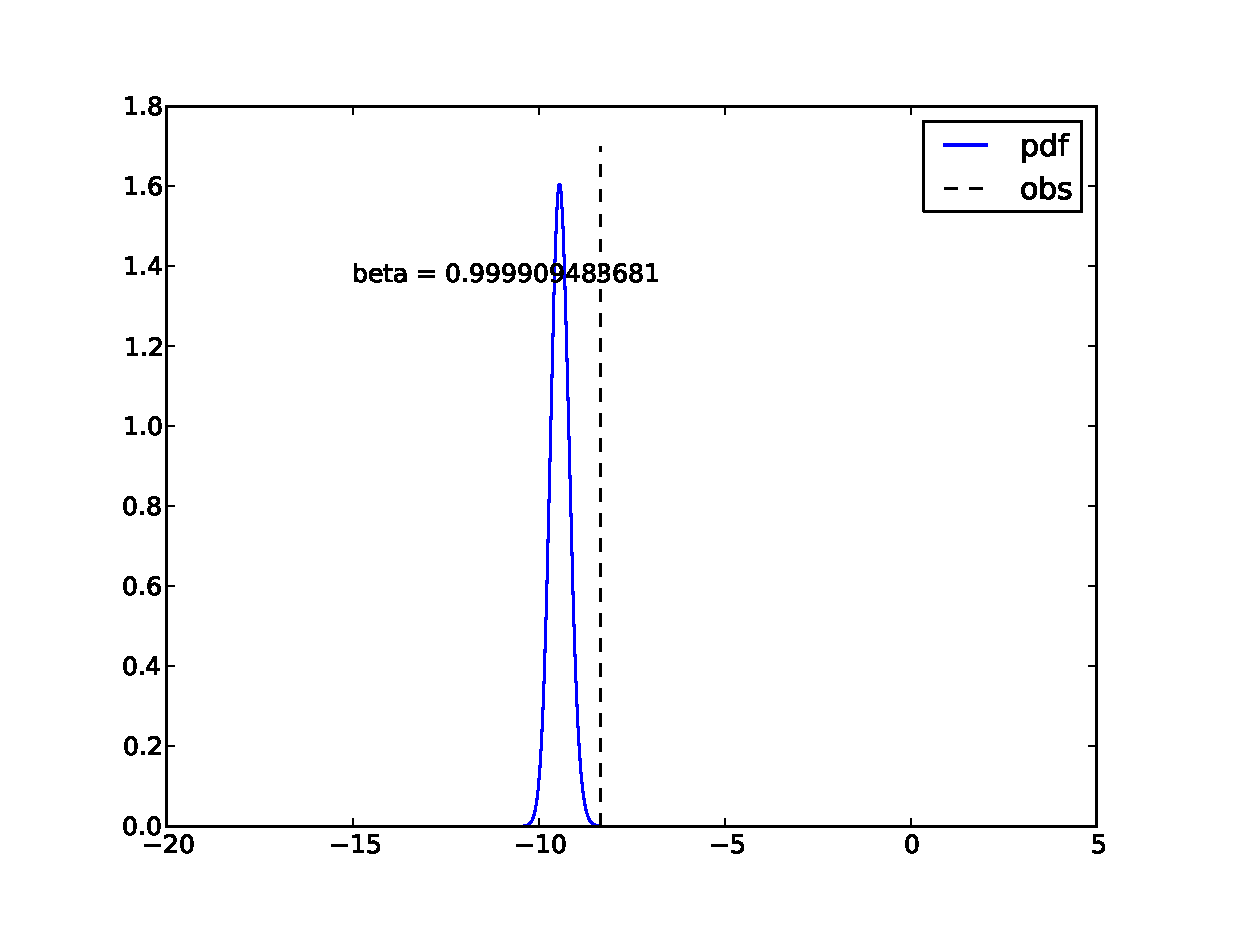
\includegraphics[width=6cm]{figs/Bowling_Ball_2_maxbeta20}}\,\,\,\subfigure[]{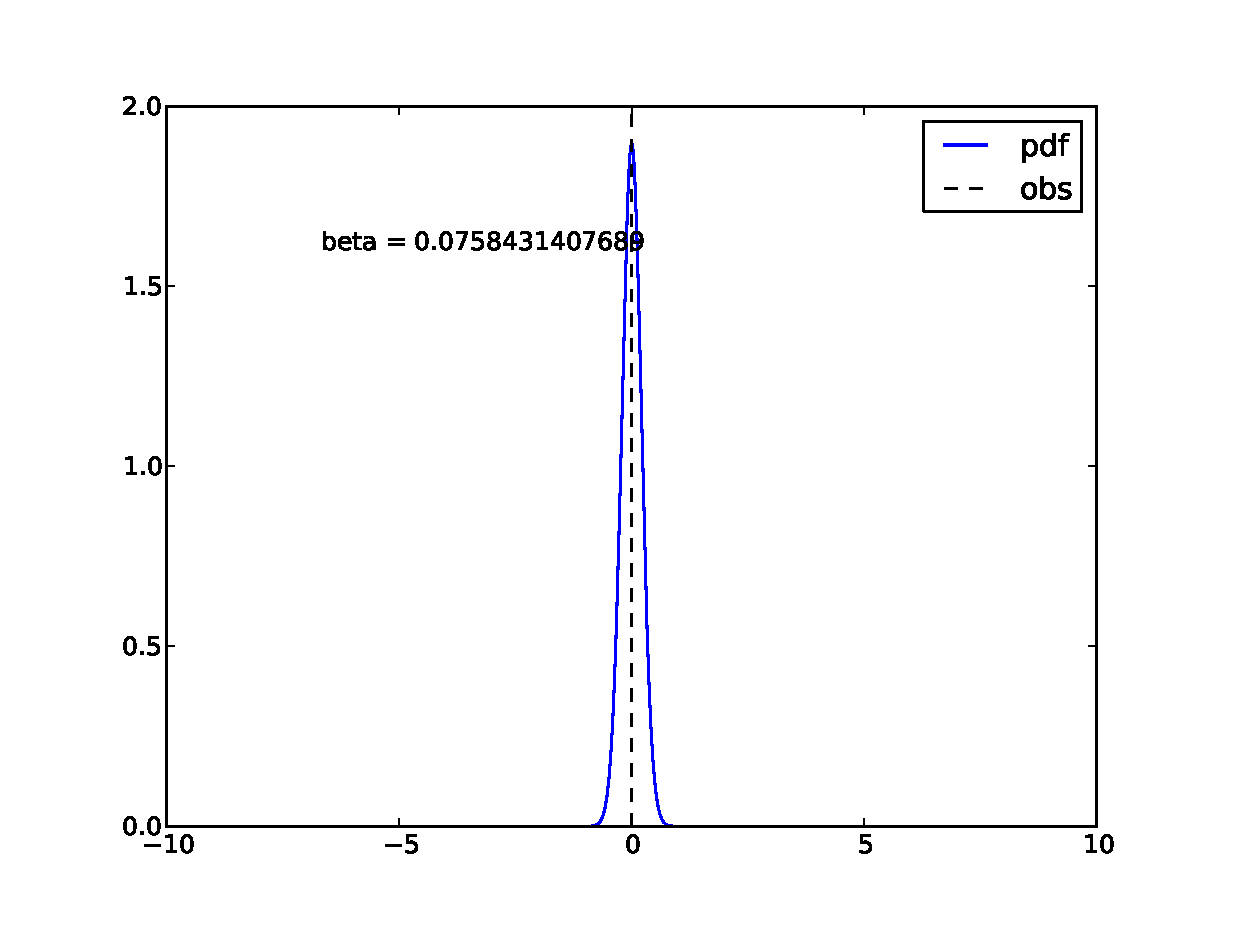
\includegraphics[width=6cm]{figs/Bowling_Ball_2_minbeta0}}
\par\end{centering}
\caption{Predicted posterior distribution at (a) maximum $\beta$ (b) minimum
$\beta$}

\label{balldrop1t5-3-3}
\end{figure}



\section{Consistency of the model}

Given the results of the above validation calculations, is the model
consistent with the observations for all drops? If not, what might
be wrong?

\subsubsection*{Solution}

From the above results, the model is clearly not consistent with the
observations for all ball drops. Rather, the model is accurate for
a finite time horizon, after which the predictions are no longer accurate.
Possible reasons for the model failure:
\begin{enumerate}
\item The assumptions made in the model may not be accurate. For
      instance, the ball may not be starting at rest, but with a
      non-zero downward velocity. 
\item The model may be inadequate, without rich enough physics to
      capture all the significant dynamics. 
\item The measurement data may not be reliable
\item The scenario parameters may have been inaccurate: for instance,
      the height of the bridge, or the size of the basketball.
\end{enumerate}

In addition, we note that the model appears to be systematically
overestimating the balls drop rate. In other words, it appears as if our
predictions are consistently projecting the ball to fall farther than it
actually does. This hints that our drag model may be at fault, because
it is not reducing the rate at which the ball falls as much as will in
reality. 

\end{document}
